% IMPORT SETTINGS
\documentclass[11pt,a4paper,twoside,openright]{report}
% CREATED BY DAVID FRISK, 2016

% BASIC SETTINGS
\usepackage{moreverb}								% List settings
\usepackage{textcomp}								% Fonts, symbols etc.
\usepackage{lmodern}								% Latin modern font
\usepackage{helvet}									% Enables font switching
\usepackage[T1]{fontenc}							% Output settings
\usepackage[english]{babel}							% Language settings
\usepackage[utf8]{inputenc}							% Input settings
\usepackage{amsmath}								% Mathematical expressions (American mathematical society)
\usepackage{amssymb}								% Mathematical symbols (American mathematical society)
\usepackage{graphicx}								% Figures
\usepackage{subfig}									% Enables subfigures
\numberwithin{equation}{chapter}					% Numbering order for equations
\numberwithin{figure}{chapter}						% Numbering order for figures
\numberwithin{table}{chapter}						% Numbering order for tables
\usepackage{listings}								% Enables source code listings
\usepackage{chemfig}								% Chemical structures
\usepackage[top=3cm, bottom=3cm,
			inner=3cm, outer=3cm]{geometry}			% Page margin lengths			
\usepackage{eso-pic}								% Create cover page background
\newcommand{\backgroundpic}[3]{
	\put(#1,#2){
	\parbox[b][\paperheight]{\paperwidth}{
	\centering
	\includegraphics[width=\paperwidth,height=\paperheight,keepaspectratio]{#3}}}}
\usepackage{float} 									% Enables object position enforcement using [H]
\usepackage{parskip}% Enables vertical spaces correctly 
\setlength{\parskip}{1em}
\usepackage{bbm}
\usepackage{mathrsfs}



%\usepackage{include/settings/standard}


% OPTIONAL SETTINGS (DELETE OR COMMENT TO SUPRESS)


% Caption settings (aligned left with bold name)
\usepackage[labelfont=bf, textfont=normal,
			justification=centering,
			singlelinecheck=false]{caption} 		

		  	
% Activate clickable links in table of contents  	
\usepackage{hyperref}								
\hypersetup{colorlinks, citecolor=blue,
   		 	filecolor=black, linkcolor=black,
    		urlcolor=blue}


% Define the number of section levels to be included in the t.o.c. and numbered	(3 is default)	
\setcounter{tocdepth}{5}							
\setcounter{secnumdepth}{5}	


% Chapter title settings
\usepackage{titlesec}		
\titleformat{\chapter}[display]
  {\Huge\bfseries\filcenter}
  {{\fontsize{50pt}{1em}\vspace{-4.2ex}\selectfont \textnormal{\thechapter}}}{1ex}{}[]


% Header and footer settings (Select TWOSIDE or ONESIDE layout below)
\usepackage{fancyhdr}								
\pagestyle{fancy}  
\renewcommand{\chaptermark}[1]{\markboth{\thechapter.\space#1}{}} 


% Select one-sided (1) or two-sided (2) page numbering
\def\layout{2}	% Choose 1 for one-sided or 2 for two-sided layout
% Conditional expression based on the layout choice
\ifnum\layout=2	% Two-sided
    \fancyhf{}			 						
	\fancyhead[LE,RO]{\nouppercase{ \leftmark}}
	\fancyfoot[LE,RO]{\thepage}
	\fancypagestyle{plain}{			% Redefine the plain page style
	\fancyhf{}
	\renewcommand{\headrulewidth}{0pt} 		
	\fancyfoot[LE,RO]{\thepage}}	
\else			% One-sided  	
  	\fancyhf{}					
	\fancyhead[C]{\nouppercase{ \leftmark}}
	\fancyfoot[C]{\thepage}
\fi


% Enable To-do notes
\usepackage[textsize=tiny]{todonotes}   % Include the option "disable" to hide all notes
\setlength{\marginparwidth}{2.5cm} 


% Supress warning from Texmaker about headheight
\setlength{\headheight}{15pt}		





%Added by me 
%%%%%Bibliography%%%%%
\usepackage[style=numeric,sorting=none,maxbibnames=5]{biblatex}
\addbibresource{include/backmatter/references.bib}
\usepackage{csquotes}
%%%%%%%%%%%%%%%%%%%%%%%
\usepackage{tensor}
\usepackage{units}
%\usepackage{cite}
\usepackage{stmaryrd}%llandrrbrackets
%\usepackage{packages/Dynkin/dynkin-diagrams}
\usepackage{tikz}
\usepackage{include/settings/TikzDrawings}
\usetikzlibrary{arrows}
\usetikzlibrary{matrix}
\usepackage{slashed}% Dirac slash


%\newcommand{\eqref}[1]{\text{(\ref{#1})}} % Make correct equation reference
\newcommand{\figref}{\figurename~\ref} 
\newcommand{\tabref}{\tablename~\ref} 
\newcommand{\apxref}{\appendixname~\ref}


%%Det ska vara ett rakt µ i prefixet
\usepackage{upgreek}
\newcommand{\micro}{\ifmmode\upmu\else$\upmu$\fi}
%%Ohm enhetskommando
\newcommand{\ohm}{\ifmmode\Upomega\else$\Upomega$\fi}


\usepackage{bbm}
\newcommand{\La}{\mathcal{L}} % Lagrangian
\newcommand{\ii}{\mathrm{i}} % Vertical i 
\newcommand{\ee}{\mathrm{e}} % Vertical e 
\newcommand{\R}{\ensuremath{\mathbbm{R}}}
\newcommand{\Or}[1]{\ensuremath{\mathcal{O}}\left(#1\right)}

\newcommand{\lp}{\ensuremath{\left(}}
\newcommand{\rp}{\ensuremath{\right)}}
\newcommand{\pd}{\ensuremath{\partial}}

\newcommand{\degC}{\ifmmode \,^\circ\mathrm{C} \else $\,^\circ\mathrm{C}$ \fi}
\newcommand{\Comm}[2]{\left[#1\,,\,\, #2\right]}
\newcommand{\DComm}[2]{\llbracket#1\,,\,\, #2\rrbracket]}
\newcommand{\aComm}[2]{\left\{#1\,,\,\, #2\right\}}



\newcommand{\dt}{\mathrm{dt}}
\newcommand{\dtt}{\mathrm{d}\tau}
\newcommand{\dx}{\mathrm{dx}}
\newcommand{\dy}{\mathrm{dy}}
\newcommand{\dz}{\mathrm{dz}}
\newcommand{\dd}{\mathrm{d}}
\newcommand{\Ricciscalar}{\ensuremath{\mathcal{R}}}
\newcommand{\Lie}{\ensuremath{\mathscr{L}}}


\newcommand{\overbar}[1]{\mkern 1.5mu\overline{\mkern-1.5mu#1\mkern-1.5mu}\mkern 1.5mu}%Appropriately sized overbar





\begin{document} 

% COVER PAGE, TITLE PAGE AND IMPRINT PAGE
\pagenumbering{roman}			% Roman numbering (starting with i (one)) until first main chapter
% CREATED BY DAVID FRISK, 2016

% COVER PAGE
\begin{titlepage}
\newgeometry{top=3cm, bottom=3cm,
			left=2.25 cm, right=2.25cm}	% Temporarily change margins		
			
% Cover page background 
\AddToShipoutPicture*{\backgroundpic{-4}{56.7}{figure/auxiliary/frontpage_eng.pdf}}
\addtolength{\voffset}{2cm}

% Cover picture (replace with your own or delete)		
\begin{figure}[H]
\centering
\vspace{2cm}	% Adjust vertical spacing here
%
\includegraphics[width=0.5\textwidth]{figure/CB.png}
\BigPicture{0.8}
\end{figure}


%Title and subtitle
\newcommand{\headtitle}{Extended geometries}
\newcommand{\subtitle}{Extensions of geometry motivated by the symmetries of string theory/M-theory}


% Cover text
\mbox{}
\vfill
\renewcommand{\familydefault}{\sfdefault} \normalfont % Set cover page font
\textbf{{\Huge 	\headtitle}} 	\\[0.5cm]
{\Large }\\[0.5cm]
Master's thesis in Physics and Astronomy \setlength{\parskip}{1cm}

{\Large ROBIN KARLSSON} \setlength{\parskip}{2.9cm}

Department of Physics \\
\textsc{Chalmers University of Technology} \\
Gothenburg, Sweden 2018

\renewcommand{\familydefault}{\rmdefault} \normalfont % Reset standard font
\end{titlepage}


% BACK OF COVER PAGE (BLANK PAGE)
\newpage
\restoregeometry
\thispagestyle{empty}
\mbox{}


% TITLE PAGE
\newpage
\thispagestyle{empty}
\begin{center}
	\textsc{\large Master's thesis 2018:NN}\\[4cm]		% Report number given by department 
	\textbf{{\Huge 	Extended geometries}} 	\\[1cm]
	{\large Extensions of geometry motivated by the symmetries of string theory/M-theory}\\[1cm]
	{\large ROBIN KARLSSON}
	
	\vfill	
	% Logotype on titlepage	
	\begin{figure}[H]
	\centering
	% Remove the following line to remove the titlepage logotype
	
\includegraphics[width=0.2\pdfpagewidth]{figure/auxiliary/logo_eng.pdf} \\	
	\end{figure}	\vspace{5mm}	
	
	Department of Physics \\
	\emph{Division of Theoretical Physics}\\
	%Name of research group (if applicable)\\
	\textsc{Chalmers University of Technology} \\
	Gothenburg, Sweden 2018 \\
\end{center}


% IMPRINT PAGE (BACK OF TITLE PAGE)
\newpage
\thispagestyle{plain}
\vspace*{4.5cm}
Extended geometries\\
Extensions of geometry motivated by the symmetries of string theory/M-theory\\
ROBIN KARLSSON \setlength{\parskip}{1cm}

\copyright ~ ROBIN KARLSSON, 2018. \setlength{\parskip}{1cm}

Supervisor: Martin Cederwall, Department of Physics\\
Examiner: Martin Cederwall, Department of Physics \setlength{\parskip}{1cm}

Master's Thesis 2018:NN\\	% Report number given by department 
Department of Physics\\
Division of Theoretical Physics\\
%Name of research group (if applicable)\\
Chalmers University of Technology\\
SE-412 96 Gothenburg\\
Telephone +46 31 772 1000 \setlength{\parskip}{0.5cm}

\vfill
% Caption for cover page figure if used, possibly with reference to further information in the report
Cover: Schematic diagram of \emph{some} of the relations between M-theory, string theories (ellipses), supergravity theories and extended geometries. \setlength{\parskip}{0.5cm}

Typeset in \LaTeX \\
Printed by [Name of printing company]\\
Gothenburg, Sweden 2018



% ABSTRACT
\newpage
% CREATED BY DAVID FRISK, 2016
Extended geometries\\
Extensions of geometry motivated by the symmetries of string theory/M-theory\\
ROBIN KARLSSON\\
Department of Physics\\
Chalmers University of Technology \setlength{\parskip}{0.5cm}

\thispagestyle{plain}			% Supress header 
\setlength{\parskip}{0pt plus 1.0pt}
\section*{Abstract}
The low-energy effective field theories of string theory/M-theory compactified on torii posses ``hidden'' symmetries by the exceptional Lie groups. Moreover a discrete version, U-duality, appears to be unbroken in the full theory. Generically such transformations mix gravitational and non-gravitational degrees of freedom and a covariant formalism calls for a merger of the underlying fields. The goal of extended geometries is therefore to generalise ordinary geometry in order to include non-gravitational degrees of freedom as a part of an extended geometry. This is done by introducing spacetime coordinates in a module of an arbritrary structure group which do effectively merge gravity with other fields. The physically most interesting cases are double field theory and exceptional field theory which are introduced before the general construction of extended geometries. Especially we focus on closure of the algebra of generalised diffeomorphisms which for consistency requires a local embedding of ordinary geometry. Moreover, an invariant action for the generalised metric is derived as well as geometrical objects such as torsion and a generalised Ricci-tensor. Lastly a specific sector of an extended geometry based on the rank seven exceptional group is used to study some properties of flux compactifications from eleven dimensional supergravity to four dimensions. 



%In general such symmetry transformations mix gravitational and non-gravitational degrees of freedom and the goal of exceptional geometry is to unify these fields by generalising the notion of geometry. Extended geometry is a general construction, 
%Extended geometries aims to include such extra degrees of freedom 
%include these symmetries as a part of the underlying geometry by extending spacetime to transform in a module of an extended structure group. The physically most interesting cases are geometries based on structure groups being the exceptional Lie groups which 


%Moreover, we look at 


%A different approach of exceptional generalised geometry making the exceptional groups manifest in supergravity is also discussed. This is also used to study some details of flux compactifications rather naturally. 

% KEYWORDS (MAXIMUM 10 WORDS)
\vfill
Keywords: Extended geometry, U-duality, M-theory, symmetries, compactification.

\newpage				% Create empty back of side
\thispagestyle{empty}
\mbox{}

% ACKNOWLEDGEMENTS
\newpage
% CREATED BY DAVID FRISK, 2016
\thispagestyle{plain}			% Supress header
\section*{Acknowledgements}
Lorem ipsum dolor sit amet, consectetur adipisicing elit, sed do eiusmod tempor incididunt ut labore et dolore magna aliqua. Ut enim ad minim veniam, quis nostrud exercitation ullamco laboris nisi ut aliquip ex ea commodo consequat. Duis aute irure dolor in reprehenderit in voluptate velit esse cillum dolore eu fugiat nulla pariatur. Excepteur sint occaecat cupidatat non proident, sunt in culpa qui officia deserunt mollit anim id est laborum.

\vspace{1.5cm}
\hfill
Robin Karlsson, Gothenburg, June 2018

\newpage				% Create empty back of side
\thispagestyle{empty}
\mbox{}


% TABLE OF CONTENTS
\newpage
\tableofcontents

% OTHER FRONTMATTER
% List of figures (add to table of contents)
\cleardoublepage
\addcontentsline{toc}{chapter}{\listfigurename} 
\listoffigures
% List of tables (add to table of contents)
\cleardoublepage
\addcontentsline{toc}{chapter}{\listtablename}  
\listoftables


% START OF MAIN DOCUMENT
\cleardoublepage
\setcounter{page}{1}
\pagenumbering{arabic}			% Arabic numbering starting from 1 (one)
\setlength{\parskip}{10pt}
\setlength{\parindent}{10pt}


\chapter{Introduction}
During the 20th century fundamental physics split into two overarching categories: quantum physics governing the subatomic world through the strong-, weak- and electromagnetic force and the theory of general relativity describing gravity. The latter tells the story of gravity warping spacetime such that an object in it follows a geodesic, the shortest path in a curved space. On the other hand we have the other three forces. These are described by Quantum field theories, were particles arise as excitations of a quantized field. This framework works extraordinarily well to high precision tested by particle accelerators around the world, e.g.\ at Large Hadron Collider at CERN Geneva.

The theory of general relativity allows for black hole solutions, which are an object so dense that nothing can escape its gravitational pull once it enters inside the so called event horizon. These strange objects that have created a lot of controversy during the last century have recently, roughly 100 years after the discovery of general relativity, been discovered directly through gravitational waves emitted from two merging black holes. Indirectly they have been observed and puzzled people for quite some time. At the moment little is known about the fate of the singularity inside a black hole.

Quantum field theory is conventionally placed in a flat spacetime, in agreement with Einsteins ingenious equivalence principle stating roughly that in a sufficiently small region spacetime looks flat and the fact that the force of gravity is many order of magnitudes weaker than the other forces. However, a black hole presents a region of spacetime where gravity is very strong due its immense density and one should therefore start to worry about quantum effects and gravity being of similar strength. Stephen Hawking was one who thought about this and reached the conclusion that quantum effects would lead evaporation of the black hole, in stark contradiction to the classical result.

Except for gravity the development has been to take a theory, say electromagnetism coupling to matter, and quantize fields of the theory. One would therefore hope to do the same with the gravitational field, however, this turns out to be incredibly hard and pathological. Quantizing relativity turns out to give a so called non-renormalizable theory unable to predict physical observables in contrast the renormalizable theories of the other forces. 

A common tool for fundamental physics during the last 100 years have been the use of symmetries. The standard model of particle physics relies on the gauge group $SU(3)\times SU(2)\times U(1)$, without this symmetry the theory would lose its predictive power. In fact, the particle spectrum is in some sense determined by ensuring that these symmetries hold non-perturbatively through so-called anomaly cancellations. General relativity on the other hand is governed by the symmetry of diffeomorphism invariance, which roughly speaking implies that the laws of physics looks the same in an arbitrary coordinate system. 

The quantization of gravity, quantum gravity, has been an ongoing field of research for many years. One of the most promising frameworks are string theory. String theory replace the notion of the most fundamental objects as pointlike to be a 1-dimensional extended object, a string. Oscillations of strings are interpreted as different particles, of which it turns out that the graviton, the particle mediating gravity, is present in any consistent string theory. Extended objects perceive the physical world quite different than particles which seems to make the theory more well behaved than that for their pointlike counterparts. However, one striking implication of string theory is that it can be consistently formulated in ten spacetime dimensions only, which seems to be in contradiction with our everyday experience of four dimensions. One way of dealing with this is the idea of compactification, where certain spacelike directions are ``small'' compared to the others, such that the effective dimension perceived is lower. 

Five consistent theories of string has been developed: Type I, Type IIA/B and two heterotic string theories. These were thought to be five inequivalent theories and the hope was that one of them should describe our physical world. However, it was argued by Witten \cite{WittenDualities1995} that they all were in fact related to each other in certain ways, through dualities. Even more so, their description at low energies could all be related to a theory in 11 dimensions dubbed M-theory. This theory in one dimension higher is known at low energies while the full theory still remains unknown.


Dualities mix gravity and other degrees of freedom which points to a unification amongst them. Due to this the notion of geometry needs to be generalised in order to account for non-gravitational degrees of freedom as well. Extended geometries in this thesis describe a generalisation of ordinary geometry to include dualities as manifest symmetries of the theory. 

\section{Outline}

\chapter{Symmetry algebras}\label{chap:symmetries}
A cornerstone of extended geometries and any fundamental theory of physics is symmetry. Hence, this chapter aims to introduce the corresponding mathematics describing these symmetries, especially Lie algebras and its representation theory. In order to construct extended geometries we need, in particular, to understand Dynkin diagrams, weights and representation theory. Moreover, we extend the finite dimensional Lie algebras to certain infinite dimensional algebras, Kac-Moody algebras as well as Borcherds superalgebras, which encode important information about the theory. 

Finite dimensional simple Lie algebras has been completely classified and comes in four different (infinite) families 
\begin{equation*}
    \mathfrak{a}_{n-1} \cong \mathfrak{sl}_{n},\quad \mathfrak{b}_{n}\cong \mathfrak{so}_{2n+1},\quad \mathfrak{c}_{n} \cong \mathfrak{sp}_{2n},\quad \mathfrak{d}_{n}\cong \mathfrak{so}_{2n},
\end{equation*}
together with five exceptional algebras
\begin{equation*}
    \mathfrak{g}_2,\quad \mathfrak{f}_4,\quad\mathfrak{e_6},\quad \mathfrak{e_7},\quad \mathfrak{e_8}.
\end{equation*}
The Lie groups corresponding to the infinite families of algebras above are related to matrix groups while the exceptional algebras can not be expressed as matrices. The two main examples that are of interest in this thesis are the $\mathfrak{so}_{2n}$ and the so-called e-series $\mathfrak{e}_n$. The general construction of extended geometries is, however, based on an arbitrary Kac-Moody algebra $\mathfrak{g}$. 

A complete introduction to the theory of Lie algebras is beyond the scope of this thesis. Instead the goal is to introduce main concepts that are of interest later on. For a thorough introduction to finite-dimensional Lie algebras we refer to \cite{Fuchs1997,FultonHarris2004,Gaberdiel2013} and for infinite-dimensional algebras \cite{Kac1990}. In section \ref{sec:groups} Lie groups, representations and how to retrieve the corresponding Lie algebra is reviewed. The theory of Lie algebras is then introduced in section \ref{sec:Liealgebras}. Extensions of finite dimensional Lie algebras to Kac-Moody algebras and to Borcherds superalgebras is then described in section \ref{sec:KacMoody} and \ref{sec:Borcherds} respectively. Two specific example of extended algebras is introduced which is used later on for the construction of extended geometries. The appearance of these kinds of extended symmetry algebras in string theory and supergravity is further presented in \cite{CederwallPalmkvistSuperalgebras2015,Aldazabal2014,Palmkvist2015ExpGeomSuperAlg,deWitTensorHierarchies2008}.



\section{Lie groups and their connection to Lie algebras}\label{sec:groups}
A group is simply a set $G$ together with an associative multiplication rule `$\cdot$' such that the following properties hold\footnote{We denote groups with capital letters $G$ and algebras with the $\mathfrak{mathfrak}$ font, e.g.\ $\mathfrak{g}$.} (for any $g,h,k\in G$)
\begin{align*}
    g\cdot \left(h\cdot k\right) = \left(g\cdot h\right)\cdot k, \qquad &\text{(associativity)}\\
    \exists\, e \in G \qquad \text{s.t.} \qquad e\cdot g = g = g \cdot e,\qquad &\text{(unit element)}\\
    \exists\, g^{-1}\in G\qquad \text{s.t.}\qquad g^{-1}\cdot g = e = g\cdot g^{-1}. \qquad &\text{(inverse element)}
\end{align*}
These axioms are natural properties of symmetry transformations which motivates the use of groups to describe symmetries. The main interest in this thesis will be in continuous infinite-dimensional groups called \emph{Lie groups}. 


A Lie group $G$ is a group which is also a differentiable manifold together with a group operation which is smooth. A typical example of such a group is $SO(3)$ describing rotations in three dimensions. Elements in the group acts as symmetry operations on physical objects such as fields and how they act is described by a \emph{representation} ($\rho,\mathbb{V}$)\footnote{Quite often a ``representation'' is interchangeably used for $\rho$ and $\mathbb{V}$, we adopt to this as it is usually clear from context what is meant.}, where $\mathbb{V}$ is a module (vector space) on which the group acts according to the linear map $\rho$. The map $\rho$ is further an homomorphism such that for $g_1,g_2\in G$
\begin{equation}
    \rho : G\to \text{Aut}(\mathbb{V}) \qquad \rho(g_1\cdot g_2) = \rho(g_1)\circ\rho(g_2),
\end{equation}
where `$\cdot$' denotes group multiplication and `$\circ$' composition of linear maps (matrix multiplication for finite-dimensional $\mathbb{V}$). A subrepresentation $\mathbb{W}\subset\mathbb{V}$ is a subspace that is preserved under the action of $G$, i.e.\
\begin{equation}
    \rho(g)w \in \mathbb{W} \qquad \text{for any} \quad g\in G,\quad w\in\mathbb{W}.
\end{equation}
Importantly, a representation is called irreducible if it does not contain any subrepresentation except for the trivial representation $\{0\}$ and $\mathbb{V}$ itself. Given two representations $(\rho_1,\mathbb{V}_1)$ and $(\rho_2,\mathbb{V}_2)$ it is possible to build two new representations, the direct sum representation and the tensor product representation
\begin{align}
    &(\mathbb{V}_1\oplus\mathbb{V}_2,\rho_{\oplus}),\qquad \rho_\oplus: g\mapsto \rho_1(g)\oplus\rho_2(g),\\
    &(\mathbb{V}_1\otimes\mathbb{V}_2,\rho_{\otimes}),\qquad \rho_\otimes: g\mapsto \rho_1(g)\otimes\rho_2(g).
\end{align}

Moreover, a representation is called indecomposable if can not be described as a direct sum of representations. Irreducible and indecomposable representations are thus ``building'' blocks for a general representation. Note that a decomposable representation is reducible while a reducible representation need not be decomposable. However, in the cases we are looking at reducible representations will be decomposable. A given tensor product representation of two irreducible representations $R_1$ and $R_2$ can then be decomposed as a direct sum of irreducible representations $R_i$ as
\begin{equation}
    R_1\otimes R_2 = \bigoplus_i R_i.
\end{equation}



In general a Lie group is a curved manifold which makes it somewhat difficult to work with. As such it is often beneficial to linearize and look at infinitesimal transformations at the identity element. Lets therefore look at the case when $G\in \text{Aut}(\mathbb{V})$, i.e.\ $G$ is a matrix group, and take $t\in [-a,a]$ with $a\in\mathbb{R_+}$ and the set of curves $\gamma(t): [-a,a]\to G$ such that $\gamma(0)= e\in G$. The tangent space at the identity $T_\mathrm{e}G$ then consist of elements $\tilde{g}$ in the corresponding \emph{Lie algebra}
\begin{equation}
\tilde{g} = \frac{\dd}{\dd t}\gamma(t)|_{t=0}.
\end{equation}
What is gained is that the tangent space $T_\mathrm{e}G$ is a vector space which in most situations are easier to deal with. Moreover, the dimension of the Lie algebra is determined by the dimensions of the manifold $G$. On the other hand one also introduce the exponential map $\text{exp}: \mathfrak{g}\to G$ in order to retrieve to group. For matrix group this map is simply the exponential of matrices in the usual sense, hence the name. Note that the topology of the group becomes important when going from the algebra to the group. For a compact connected group $G$ the exponential map is onto such that any element in $G$ can be written using elements of the algebra. On the other hand for a compact group that is not connected only the connected part can be reached. 

The group $G$ carries an representation on the Lie algebra called the Adjoint representation $\text{Ad}: G\to \text{Aut}(\mathfrak{g})$ by $g\in G$ and $\tilde{g}\in\mathfrak{g}$ acting as
\begin{equation}\label{eq:Liegrouprep}
    \text{Ad}_g(\tilde{g}) = g\tilde{g}g^{-1}.
\end{equation}
This is well-defined since the elements of the group acts naturally on the curve $\gamma$ used to define $\tilde{g}$. In the same spirit we can look at the action of a curve passing through the identity element acting on $\mathfrak{g}$ with $h,\tilde{g}\in \mathfrak{g}$ which defines the adjoint action of the algebra 
\begin{equation}
    \text{ad}(h): \mathfrak{g}\to \text{End}(\mathfrak{g}),\qquad h\mapsto \text{ad}(h)(\tilde{g}),
\end{equation}
according to 
\begin{equation}
    \text{ad}(h)(g) = \frac{\dd}{\dd t}\gamma_h(t)\tilde{g}\gamma_h^{-1}(t)|_{t=0}.
\end{equation}
It is then easily seen that on matrix algebras the adjoint action acts as a commutator 
\begin{equation}
    \text{ad}(h)(g) = [h,g],
\end{equation}
which equips the tangent space with an anti-symmetric bilinear product, hence defining an algebra. 

\section{Lie algebras}\label{sec:Liealgebras}
A Lie algebra $\mathfrak{g}$ is a vector space with an anti-symmetric bilinear product called the Lie bracket $\llbracket\cdot,\cdot\rrbracket: \mathfrak{g}\times\mathfrak{g}\to\mathfrak{g}$ that satisfies the Jacobi identity $a,b,c\in\mathfrak{g}$
\begin{equation}
\llbracket a,\llbracket b,c\rrbracket\rrbracket+\llbracket b,\llbracket c,a\rrbracket\rrbracket+\llbracket c,\llbracket a,b\rrbracket\rrbracket=0, 
\end{equation}
which can easily be seen to be true for matrix commutators. Note that the Lie bracket is non-associative, in fact the Jacobi identity can be seen as condition to ensure associtativity of the Lie group. A representation of the algebra is given by a module $\mathbb{V}$ and a map $\rho: \mathfrak{g}\to \text{End}(\mathbb{V})$ which satisfies
\begin{equation}\label{eq:lierep}
    \rho(\llbracket a,b\rrbracket) = [\rho(a),\rho(b)],
\end{equation}
where $[\cdot,\cdot]$ denotes the matrix commutator. This differs from the property of a representation for the group, but follows from consistency with eq.\ \eqref{eq:Liegrouprep}. As for groups there is a tensor product representation for Lie algebras. Given two representations the tensor product representation is defined by the module $\mathbb{V}_1\otimes\mathbb{V}_2$, with an action given by 
\begin{equation}
    \begin{aligned}
        \rho_\otimes:\quad &\mathfrak{g}\to\text{End}\left(\mathbb{V}_1\otimes\mathbb{V}_2\right), \\
                & g\mapsto \rho_1(g)\otimes \mathbf{1}+\mathbf{1}\otimes\rho_2(g),
    \end{aligned}
\end{equation}
where $\mathbf{1}$ is the identity matrix.


Being a vector space it is possible to introduce a basis $T^a$, where $a=1,2,\ldots,\text{dim}\,\mathfrak{g}$, and write the Lie bracket as 
\begin{equation}
    \llbracket T^a,T^b\rrbracket = \tensor{f}{^{ab}_c} T^c,
\end{equation}
where repeated indices is summed over. The $\tensor{f}{^{ab}_c}$ is called the structure constants and specifies the algebra. If the structure constants vanish the algebra is called abelian.

A subset $\mathfrak{h}\subset \mathfrak{g}$ is a subalgebra of $\mathfrak{g}$ if \begin{equation}
    \llbracket\mathfrak{h},\mathfrak{h}\rrbracket\subseteq \mathfrak{h},
\end{equation} 
and it is called an invariant subalgebra, or ideal, if also
\begin{equation}
    \llbracket\mathfrak{h},\mathfrak{g}\rrbracket\subseteq \mathfrak{h}.
\end{equation}
This give the important notion of simple and semi-simple algebras: a semi-simple algebra is an algebra with no abelian ideals and a simple algebra on the other hand is an algebra containing no proper ideals (i.e.\ no ideals other than the $\{0\}$ and $\mathfrak{g}$ itself). Simple algebras can then be used as building blocks for more general algebras, for example the Lie algebra related to the standard model of particle physics with gauge group $SU(3)\times SU(2)\times U(1)$ is given by $\mathfrak{g}=\mathfrak{su}(3)\oplus\mathfrak{su}(2)\oplus\mathfrak{u}(1)$, where each component is a simple algebra. 

So far the algebras have been implicitly assumed real, i.e.\ real linear combinations of elements in the vector space. Note, however, that the matrix algebras such as $\mathfrak{su}(2)$ still contains complex entries. It is often convenient to extend the field ($\mathbb{R}\to\mathbb{C}$) and allow for complex linear combinations instead, which we will do from now on unless specified otherwise. One of the consequences of this is that algebras that are inequivalent over $\mathbb{R}$ could be the equivalent upon complexification, e.g.\ $\mathfrak{su}(2)_\mathbb{C}\cong \mathfrak{sl}(2,\mathbb{C})$ while $\mathfrak{su}(2)_\mathbb{R}\ncong\mathfrak{sl}(2,\mathbb{\mathbb{R}})$. 

An important object is the symmetric invariant bilinear form of a simple Lie algebra called the Killing form. Given a representation $\rho$ the Killing form is given by 
\begin{equation}
    \kappa(T^a,T^b) := \kappa^{ab} = \frac{1}{I_\rho}\text{Tr}\left(\rho(T^a)\rho(T^b)\right),
\end{equation}
where $I_\rho$ is a normalization constant that depends on the representation. Invariance of the Killing form means that for any $g,h,k\in\mathfrak{g}$ it satisfies 
\begin{equation}
    \kappa(\llbracket g,h\rrbracket,k) = \kappa(h,\llbracket g,k\rrbracket). 
\end{equation}
Interesting properties can be read of from the Killing form, e.g.\ a semi-simple algebra implies that the Killing form is non-degenerate. Moreover, if $\kappa$ is negative definite, then the algebra is called compact meaning in turn that the corresponding exponentiated Lie group is a compact manifold. Importantly one can also use the Killing form and its inverse to raise and lower adjoint indices. 


\subsection{Example -- Chevalley set}
As an example we will study $\mathfrak{a}_1\cong\mathfrak{sl}(2,\mathbb{C})$ which is an important algebra because, as we will see later, more complicated algebras can be constructed as a collection of ``interacting'' $\mathfrak{a}_1$ subalgebras. This algebra consists of $2\times 2$ traceless matrices over $\mathbb{C}$ and a possible choice of basis is
\begin{equation}
    h=\begin{pmatrix}1&0\\0 &-1\end{pmatrix},\qquad e=\begin{pmatrix}0&1\\0 &0\end{pmatrix},\qquad f=\begin{pmatrix}0&0\\1 &0\end{pmatrix}.
\end{equation}
The structure constants in this basis is easily calculated to
\begin{equation}
    [h,e] = 2e_+,\qquad [h,f]=-2e_-, \qquad [e,f]=h.
\end{equation}
Observe that the elements $e,f$ can thus be seen as step operators increasing(decreasing) the eigenvalue of $h$ by $\pm 2$. From a physicist point of view this is reminiscent of the $\{J_3,J_+,J_-\}$ basis of angular momentum in quantum mechanics and the action of the algebra is displayed in \figref{fig:SlTwoRep}. The Killing form in the fundamental representation, this is the representation with $\rho =\mathbf{1}$ for matrix algebras, is easily calculated and one finds 
\begin{equation}
    \kappa = \begin{pmatrix}2&0&0\\0&0&1\\0&1&0\end{pmatrix},
\end{equation}
with an ordering $\{h,e^+,e^-\}$. Indeed we find that $\text{det}(\kappa)\neq 0$ as claimed for a simple Lie algebra.

Suppose that we have a finite dimensional irreducible representation $\mathbb{V}$. Then due to the commutation relations one finds that $h$ acts diagonally on vectors $v\in \mathbb{V}$ and can therefore be decomposed into eigenspaces of $h$ according to
\begin{equation}
    \mathbb{V} = \bigoplus_\alpha \mathbb{V}_\alpha,
\end{equation}
where any $v\in\mathbb{V}_\alpha$ is an eigenvector of $h$ such that\footnote{Here we dropped the explicit use of $\rho(h)v :=hv$, and we will continue to do so when convenient.} $hv_\alpha = \alpha v$. As for a spin representation in quantum mechanics one deduce that possible eigenvalues are integers symmetrically distributed around the origin. A representation for $\mathfrak{a}_1$ can thus be specified by a vector $v_\lambda$, where $\lambda$ is the largest eigenvalue of $h$ on $\mathbb{V}$. The representation is then spanned by states obtained by acting with the lowering operator $f$ on $v_\lambda$ 
\begin{equation}
    \mathbb{V} = \{v_\lambda,fv_\lambda,f^2v_\lambda,\ldots,f^{n}v_\lambda\}.
\end{equation}

Note that $ev_\lambda = 0$ as well as $f(f)^{n}v_\lambda=0$, the vectors $v_\lambda$ and $(f)^{n}v_n$ are therefore called highest and lowest weight vectors respectively. The eigenvalues of $h$ on $\mathbb{V}$ is called weights, and especially, $\lambda$ is called the highest weight. 

\begin{figure}
    \centering
    \drawSlTwoRep{0.4}
    \caption{Illustration of the ``weight'' lattice for $\mathfrak{a}_1$. Action of the algebra is indicated. }
    \label{fig:SlTwoRep}
\end{figure}



\subsection{Roots, weights and representations}
Based on the $\mathfrak{a}_1$ example we will now build up the representation theory for an arbitrary simple Lie algebra $\mathfrak{g}$. The starting point is to find a maximal commuting subalgebra $\mathfrak{h}$ called the Cartan subalgebra, which in the example above this was just given by $\{h\}$. The Cartan subalgebra then act diagonally on any irreducible finite-dimensional representation $\mathbb{V}$. This property is analogous to the fact that commuting operators in quantum mechanics can be simultaneously diagonalizable. Hence, the representation can be decomposed as 
\begin{equation}
    \mathbb{V} = \bigoplus_\alpha \mathbb{V}_\alpha.
\end{equation}
Compared to the case where $\mathfrak{h}$ were one-dimensional, the eigenvalue $\alpha$ in this case is rather a vector containing the eigenvalues for each element in $\mathfrak{h}$. Another way to put it is that $\alpha\in \mathfrak{h}^*$, i.e.\ $\alpha$ is a linear functional $\alpha:\mathfrak{h}\to \mathbb{C}$. The dimension $r$ of the Cartan subalgebra is called the rank which is often denoted as a subscript on the algebra, e.g.\ $\mathfrak{g}_r$, $\mathfrak{a}_r$, $\mathfrak{e}_8$ and so on. Especially, decomposing the adjoint representation we find
\begin{equation}\label{eq:algdecomp}
    \mathfrak{g} = \mathfrak{h}\oplus\bigoplus_{\alpha\in\Delta} \mathfrak{g}_\alpha,
\end{equation}
where, by definition, for any $h\in\mathfrak{h}$ and $v_\alpha\in\mathfrak{g}_\alpha$ 
\begin{equation}
    \text{ad}_h(v_\alpha) = \alpha(h)v_\alpha.
\end{equation}
This choice of basis is called the Cartan-Weyl basis. The sum in \eqref{eq:algdecomp} is over a finite set $\Delta\subset\mathfrak{h}^*$ called the root system and the elements $\alpha\in\Delta$ are called roots. Moreover, it follows by the Jacobi-identity that 
\begin{equation}
    \text{ad}_{\mathfrak{g}_\alpha}(\mathfrak{g}_\beta) = \llbracket\mathfrak{g}_\alpha,\mathfrak{g}_\beta\rrbracket \subset \mathfrak{g}_{\alpha+\beta}.
\end{equation}
We thus see that by acting with an element in $\mathfrak{g}_\alpha$ on some other element in $\mathfrak{g}_\beta$, one can ``move'' around in the algebra, or equivalently in the adjoint representation. Acting with the Cartan subalgebra on the other hand preserves the subspace $\mathfrak{g}_\beta$. As such one defines the root lattice $\Lambda_R$, which simply is a $r$-dimensional lattice spanned by integral linear combinations of the roots $\alpha\in\Delta$. Furthermore, we split the root system $\Delta$ in to positive and negative roots as $\Delta = \Delta^+\cup\Delta^-$. This can be seen as a choice of a hyperplane in the root lattice such that it contains no roots, the set of roots thus gets divided in two disjoint unions. Intuitively the positive roots corresponds to raising operators while the negative roots acts as lowering operators. There is some arbitrariness in this choice, however, the particular choice is without significance as long as one sticks to it. There is a canonical choice of basis for the root lattice called simple roots; these are $r$ positive roots such that any positive root is obtained by non-negative linear combinations of such roots. 

The discussion above concerned the adjoint representation, let us continue to some arbitrary finite dimensional irreducible representation $\mathbb{V}$. As above this can be decomposed in to eigenspaces of $\mathfrak{h}$
\begin{equation}
    \mathbb{V} = \bigoplus_\beta \mathbb{V}_\beta,
\end{equation}
where $\beta$, called weights, lie in some finite subset of $\mathfrak{h}^*$. Using the defining property of Lie algebra representations one finds that by applying an element $e_\alpha\in\mathfrak{g}$ on $v_\alpha\in\mathbb{V}_\beta$ that 
\begin{equation}
    \rho(e_\alpha)v_\beta \in \mathbb{V}_{\alpha+\beta}.
\end{equation}
Hence, root vectors (a root vector $e_\alpha$ is a vector in the vector space with the root $\alpha$ as eigenvalue) can again be used to ``jump between'' vectors in $\mathbb{V}$ with different eigenvalues/weights as in the $\mathfrak{a}_1$ case. Moreover, using non-degeneracy of the Killing form, one can show that if $\alpha$ is a root, then also $-\alpha$ is a root. This is important since one can then construct a collection of $\mathfrak{a}_1$ subalgebras of $\mathfrak{g}$ as 
\begin{equation}
    \mathfrak{a}_1^\alpha = e_\alpha \oplus e_{-\alpha} \oplus \llbracket e_\alpha,e_{-\alpha}\rrbracket.
\end{equation}
Any representation $\mathbb{V}$ of $\mathfrak{g}$ must also be an representation of the subalgebras $\mathfrak{a}_1^\alpha$, and since the weights of $\mathfrak{a}_1$ is integer valued it follows that also the weights of any representation $\mathbb{V}$ of $\mathfrak{g}$ are integer valued, i.e.\ a weight $\beta\in\mathfrak{h}^*$ satisfies $\beta(h)\in\mathbb{Z}$ for any $h\in\mathfrak{h}$. With this one defines the weight lattice $\Lambda_W$, which is a rank $r$ lattice containing all weights $\beta$ such that $\beta(\mathfrak{h})\in\mathbb{Z}$. Any representation is therefore equivalent to a set of weights in $\Lambda_W$. 

Importantly, any irreducible finite dimensional representation can be characterized by a highest weight $\lambda$, as such we call the representation a highest weight representation. A highest weight $\lambda$ and the corresponding highest weight vector is defined such that acting with any root vector corresponding to a positive root $\alpha\in\Delta^+$ annihilates the vector
\begin{equation}
    e_\alpha v_\lambda = 0.
\end{equation}

In the $\mathfrak{a}_1$ analogy with quantum mechanics this simply corresponds to the largest $J_3$ eigenvalue with the generalisation that $\lambda$ is now a ``vector of quantum numbers''. Given any highest weight vector $v_\lambda$ the corresponding highest weight representation $\mathbb{V}$ consist of elements obtained by acting with root vectors corresponding to negative roots $\alpha\in\Delta^-$ on $v_\lambda$. Since by assumption the representation is finite dimensional and irreducible this construction eventually terminates.

The Killing form for semi-simple Lie algebras was introduced above as a non-degenerate symmetric bilinear form on the algebra. Being non-degenerate implies that it defines an inner product on $\mathfrak{g}$, and hence also an isomorphism between algebra $\mathfrak{g}$ and its dual space $\mathfrak{g}^*$. Therefore, since $\alpha\in\mathfrak{h}^*$, any root $\alpha$ is associated with an element $h_\alpha:=\alpha^\vee$ called a coroot in the Cartan subalgebra such that 
\begin{equation}\label{eq:CorootsDef}
    \beta(\alpha^\vee) = \frac{2(\alpha,\beta)}{(\alpha,\alpha)},
\end{equation}
for any $\beta\in\mathfrak{h}^*$. Moreover, this in turn can be used to define a non-degenerate inner product $(\cdot,\cdot)$ on $\mathfrak{h}^*$ according to
\begin{equation}
    (\alpha,\beta):= c_\alpha c_\beta \kappa(h_\alpha,h_\beta),
\end{equation}
for some constants $c_{\alpha,\beta}$. The coroots of simple roots $\alpha_{i}$ are called simple co-roots $\alpha_{i}^{\vee}$. Using simple co-roots a canonical basis on the weight space is given by the so called fundamental weights $\Lambda_{i}$ satisfying 
\begin{equation}\label{eq:FundWeights}
    \Lambda_i(\alpha_j^\vee) = \delta_{ij}.
\end{equation}
Any weight vector can thus be expanded in fundamental weights 
\begin{equation}
    \lambda = \sum_i \lambda_i\Lambda_{j},
\end{equation}
where the coefficients $\lambda_i$ are called Dynkin labels. An irreducible finite-dimensional module of a semi-simple Lie algebra is uniquely defined by an integral dominant highest weight $\lambda$ of multiplicity one, here integral dominant means that $\lambda_i\in \mathbb{Z}_{\geq 0}$ and multiplicity one that the vector space with vectors with weight $\lambda$ is one-dimensional.

A partial ordering is introduced between between weights as follows: given two weights $\lambda$ and $\mu$, then $\lambda>\mu$ if $\lambda-\mu$ is expressible as a non-negative linear combination of positive roots. Moreover, the height $h$ of a root $\beta$ is defined as 
\begin{equation}
    \beta = \sum_{i=1}^ra_i\alpha_i\implies h = \sum_{i=1}^r a_i.
\end{equation}
For a simple Lie algebra there exists a unique highest root, typically denoted $\theta$, such that $h_\theta>h_\alpha$, for any other root $\alpha$. Moreover, one defines the so-called Coxeter labels $a_i$ and dual Coxeter labels $a_i^\vee$ as the coefficients (up to scaling) of the highest root in simple roots and coroots respectively according to
\begin{equation}
    \theta = \sum_{i=1}^ra_i\alpha_{i},\qquad \frac{2}{(\theta,\theta)}\theta = \sum_{i=1}^r a_i^\vee \alpha_{i}^{\vee}.
\end{equation}
Yet another important object that is of interest is the so-called Weyl vector $\rho$. The Weyl vector is defined as
\begin{equation}\label{eq:Weylroots}
    \rho := \frac{1}{2}\sum_{\alpha\in\Delta^+}\alpha,
\end{equation}
and one can show that it can also be rewritten as
\begin{equation}
    \rho = \sum_{i=1}^r \Lambda_{i}.
\end{equation}

\subsection{Cartan matrix and Dynkin diagram}
We have seen that a Lie algebra is specified by its root system. Another way to characterize a Lie algebra that also is convenient for further extensions later on, is through its Cartan matrix. The $r\times r$ dimensional Cartan matrix can be obtained from the root system as
\begin{equation}\label{eq:CartanFirst}
    a_{ij} := \alpha_j(\alpha_{i}^\vee)  = \frac{2}{(\alpha_{i},\alpha_{i})}(\alpha_{i},\alpha_{j}),
\end{equation}
where $\alpha_{i}$ and $\alpha_{j}^{\vee}$ are simple roots and simple coroots respectively. In fact, a finite dimensional simple Lie algebra is completely characterized by a Cartan matrix (up to permutations) with the following properties:
\begin{equation}\label{eq:Cartanprop}
    \begin{aligned}
        a_{ii} = 2,\\
        a_{ij} = 0 \Longleftrightarrow a_{ji} = 0,\\
        a_{ij}\in \mathbb{Z}_{\leq 0} \quad\text{for}\quad i\neq j,\\
        \text{det}\, a >0,
    \end{aligned}
\end{equation}
and that it can not be written as the direct sum of such matrices. Classification of finite-dimensional simple Lie algebras thus boils down to specifying matrices with these properties. 

Starting with a Cartan matrix the corresponding algebra is then built up by $3r$ generators $\{h_i,e_i,f_i\ |i=1,2,\ldots,r\}$ subject to the constraints
\begin{equation}
\begin{aligned}\label{eq:Cartanrules}
    \llbracket h_i,h_j\rrbracket = 0,\\
    \llbracket h_i,e_j\rrbracket = a_{ij}e_{j},\\
    \llbracket h_i,f_j\rrbracket = -a_{ij}f_{j},\\
    \llbracket e_i,f_j\rrbracket = \delta_{ij}h_i,\\
    (\text{ad}_{e_i})^{1-a_{ij}}e_j = (\text{ad}_{f_i})^{1-a_{ij}}f_j = 0,
\end{aligned}
\end{equation}
with $i\neq j$ in the last relation. This is the so-called Chevalley-Serre basis which is a special example of a Cartan-Weyl basis. Moreover, the last line in \eqref{eq:Cartanrules} are called the Serre relations and the rest being the Chevalley relations. A Lie algebra built from a Cartan matrix $a$ will typically be denoted $\mathfrak{g}(a)$. To give an example, $\mathfrak{a}_2\cong \mathfrak{sl}(3)$ has the Cartan matrix
\begin{equation}
    a_\mathfrak{a_2}=\begin{bmatrix}2&-1\\-1&2\end{bmatrix},
\end{equation}
which is easily seen to fulfill the properties listed above. 

The Cartan matrix for a finite dimensional simple Lie algebra is symmetrisable, i.e.\ there exists a diagonal matrix $d$ such that 
\begin{equation}
    S = da,
\end{equation}
with $S$ a symmetric matrix. The matrix $S$ defines an inner product $(\cdot,\cdot)$ on $\mathfrak{h}^*$ and since $a_{ii}=2$ we find
\begin{equation}
    d_i = \frac{(\alpha_i,\alpha_i)}{2},
\end{equation}
such that 
\begin{equation}
    S_{ij} = \frac{a_{ij}(\alpha_i,\alpha_i)}{2}.
\end{equation}
This is defined up to an overall scale which we fix by setting $(\alpha_i,\alpha_i)=2$ for the longest simple root $\alpha_i$\footnote{This is a common convention.}. The length of the other simple roots are then determined by 
\begin{equation}
    (\alpha_j,\alpha_j) = \frac{2a_{ij}}{a_{ji}}< 2,
\end{equation}
if $i$ denotes the longest simple root. If all simple roots have the same length the Cartan matrix is already symmetric and the algebra is called simply-laced. Since $S$ is non-degenerate this defines an isomorphism between $\mathfrak{h}$ and its dual space according \eqref{eq:CorootsDef} and an inner product on $\mathfrak{h}^*$
\begin{equation}
    (\alpha_i^\vee,\alpha_j^\vee) := \frac{2\alpha_j(\alpha_i^\vee)}{(\alpha_j,\alpha_j)}.
\end{equation}
Since the pairing $\alpha_j(\alpha_i^\vee)=a_{ij}$ we find 
\begin{equation}
    (\alpha_i^\vee,\alpha_j^\vee) = (ad^{-1})_{ij} =: \hat{a}_{ij},
\end{equation}
the inner product on the Cartan subalgebra is thus given by the Cartan matrix symmetrised with $d^{-1}$ ``from the right''. Invariance of the inner product $(\cdot,\cdot)$ on $\mathfrak{h}$ can then be used to extend the inner product to the whole algebra $\mathfrak{g}(A)$. This essentially completes the reconstruction of a finite dimensional simple Lie algebra from its Cartan matrix. However, it also convenient to define an inner product on the weight space. The fundamental weights were defined as the dual basis to $\alpha^\vee_i$ in \eqref{eq:FundWeights} and the corresponding inner product on the weight space is given by the inverse matrix $\hat{a}^{-1}$ 
\begin{equation}
    (\Lambda_i,\Lambda_j) = (\hat{a}^{-1})_{ij}.
\end{equation}
The inner product of two weights $\lambda$ and $\mu$ is therefore given by 
\begin{equation}
    (\lambda,\mu) = \sum_{ij}(\hat{a}^{-1})_{ij}\lambda_i\mu_j,
\end{equation}
where $\lambda_i$ and $\mu_j$ are Dynkin labels. The matrix $\hat{a}^{-1}$ is often called the quadratic form matrix and can be found for finite simple Lie algebras in e.g.\ \cite{Fuchs1997}. 

A description of a Lie algebra in terms of its Cartan matrix also enables specifying an algebra through its so-called Dynkin diagram. A Dynkin diagram is a diagram with $r$ number of nodes connected by $\text{max}\,\{|a_{ij}|,|a_{ji}|\}$ lines. For non simply-laced algebras an arrow is denoted from $i$ to $j$ if $|a_{ij}|>|a_{ji}|$, i.e.\ towards the long root; another common convention is an open dot at the short root and a filled dot the long root. Any simple finite dimensional Lie algebra is thus described by its Dynkin diagram in \figref{fig:AllDynkin} and Chevalley-Serre relations \eqref{eq:Cartanrules}.
\begin{figure}
    \centering
    \AllDynkin
    \caption{Dynkin diagrams for finite dimensional simple Lie algebras.}
    \label{fig:AllDynkin}
\end{figure}



\subsection{Real forms}\label{sec:Realforms}
The analysis above used $\mathbb{C}$ as the underlying field. However, it is often of interest to look only at real linear combinations of elements in the algebra. Choosing a basis $T^a$, $a=1,2,\ldots, \text{dim}\,\mathfrak{g}$, it is clear that if the structure constants $\tensor{f}{^{ab}_c}$ are real, a restriction to real linear combinations is consistent. More generally, a real form $\hat{\mathfrak{g}}$ of an algebra $\mathfrak{g}$ satisfies
\begin{equation}
    \mathfrak{g} \cong \hat{\mathfrak{g}}\oplus i\hat{\mathfrak{g}},
\end{equation}
i.e.\ the complexification of $\hat{\mathfrak{g}}$ is isomorphic to $\mathfrak{g}$. A generic Lie algebra $\mathfrak{g}$ typically has several inequivalent real forms. Two real forms that can be constructed for any Lie algebra is the split real form and the compact real form.

The structure constants in the Chevalley-Serre basis are real, hence, by restricting to real linear combinations we get a real form called the \emph{split real form}. A second real form for any Lie algebra can be found by noting that on $\mathfrak{g}$ the Killing form is non-degenerate and one can introduce a basis such that 
\begin{equation}
    \kappa = \begin{pmatrix}\mathbf{1}_p& 0\\0&-\mathbf{1}_{d-p}
    \end{pmatrix},
\end{equation}
where $d$ is the dimension the algebra. It is always possible to choose $p=0$ such that $\kappa^{ab} = -\delta^{ab}$. Upon restriction to real linear combinations this defines the compact real form of $\mathfrak{g}$. Furthermore, given a real form $\hat{\mathfrak{g}}$ the $(d-p)$-dimensional subspace on which $\kappa$ is negative definite is actually a subalgebra of $\hat{\mathfrak{g}}$. This is called the \emph{maximal compact subalgebra}, typically denoted $\mathfrak{k}$, of $\hat{\mathfrak{g}}$ and it is by construction a real form. Note that in this case upon restriction to a real form we can no longer make ``Wick-rotations'' to change the signature of $\kappa$.

Later on we will deal with so called non-linear sigma models where physical fields take values in the coset group
\begin{equation}
G/H,
\end{equation}
where $G$ is the group obtained by exponentiating a split real form $\mathfrak{g}$ and $H$ is likewise the group corresponding to the maximal compact subalgebra $\mathfrak{k}$ of $\mathfrak{g}$.  

Another way to define the maximal compact subalgebra is by the so-called Chevalley involution\footnote{An involution is a Lie algebra automorphism with eigenvalue $\pm 1$.} $\omega$. The Chevalley involution is defined through its action on Chevalley generators
\begin{equation}
    \omega(h^i) = -h^i,\qquad \omega(e_i) = -e_i, \qquad \omega(f_i) = -f_-.
\end{equation}
The maximal compact subalgebra $\mathfrak{k}$ of the real form $\mathfrak{g}$ can then by defined as the subset that is pointwise fixed under $\omega$
\begin{equation}
    \mathfrak{k} = \{g\in\mathfrak{g}\,|\, \omega (g) = g \}. 
\end{equation}
With the definition of the Chevalley involution one sees that the maximal compact subalgebra therefore is spanned by $e_i-f_i$, $i=1,\ldots,r$. The algebra $\mathfrak{g}$ can thus be decomposed as 
\begin{equation}
    \mathfrak{g} = \mathfrak{p}\oplus\mathfrak{k},
\end{equation}
where $\omega$ acts as $\mp 1$ on $\mathfrak{p}$ and $\mathfrak{k}$ respectively. Note that $\mathfrak{p}$ is not an subalgebra, instead it transform in a representation of $\mathfrak{k}$ 
\begin{equation}
    \llbracket \mathfrak{p},\mathfrak{p}\rrbracket \subset \mathfrak{k},\qquad \llbracket \mathfrak{k},\mathfrak{p}\rrbracket\subset \mathfrak{p},\qquad \llbracket \mathfrak{k},\mathfrak{k}\rrbracket \subset \mathfrak{k}.
\end{equation}
Moreover, one could also decompose the algebra according to the Iwasawa decomposition 
\begin{equation}
    \mathfrak{g} = \mathfrak{k}\oplus\mathfrak{h}\oplus\mathfrak{n}_+,
\end{equation}
where $\mathfrak{n_+}$ is the subspac of positive roots. The subspace $\mathfrak{h}\oplus\mathfrak{n}_+$ is called a (positive) Borel subalgebra. 

\subsection{Invariant tensors}
Given a gauge symmetry neither the lagrangian nor any physical observable should depend on the gauge. As such one has to construct objects that transforms in the trivial representation (singlet) of the gauge group, or equivalently the corresponding algebra. Hence, in order to have a non-trivial theory one has to extract the singlet representation from tensor product representations. This is precisely done by invariant tensors, or intertwiners. Two important examples of such invariant tensors are the Killing form and the structure constants. 

Suppose we have a field $\phi^N$, $N=1,2,\ldots,\text{dim}\,R_1$, in a representation $R_1$ and a field $\psi^\alpha$, $\alpha=1,2,\ldots,\text{dim}\,R_2$, in another representation $R_2$. By definition these transform as 
\begin{equation}
    \phi^M \mapsto \tensor{R_1(T^a)}{^M_N}\phi^N \qquad \psi^\alpha\mapsto \tensor{R_2(T^a)}{^\alpha_\beta}\psi^\beta.
\end{equation}

Then the singlet contribution from the tensor product $R_1\otimes R_2$ is given by 
\begin{equation}
    t_{N\alpha}\phi^N\psi^\alpha \mapsto \tensor{R_1(T^a)}{^M_N}t_{M\alpha}\phi^N\psi^\alpha+\tensor{R_2(T^a)}{^\alpha_\beta}t_{N\alpha}\phi^N\psi^\beta ,
\end{equation}
if the tensor $t$ satisfies
\begin{equation}\label{eq:invarianttensorDef}
    \tensor{R_1(T^a)}{^M_N}t_{M\alpha}+\tensor{R_2(T^a)}{^\alpha_\beta}t_{N\alpha} = 0,
\end{equation}
and $t$ is called an invariant tensor. The condition \eqref{eq:invarianttensorDef} is easily extended to an arbitrary tensor product representation. Note, however, that finding such an invariant tensor is not always possible since not all tensor product representations include a singlet representation. In this way an underlying symmetry reduce the number of possible terms in a lagrangian. 

Given a representation $R$ and its conjugate dual $\overbar{R}$ with index $^m$ and $_m$ respectively, it is possible to create new invariant tensors from given invariant tensors by summing, taking products and contracting indices
\begin{equation}
\begin{aligned}
\tensor{t}{^{n_1\ldots}_{m_1\ldots}}+\tensor{\tilde{t}}{^{n_1\ldots}_{m_1\ldots}},\\
\tensor{t}{^{n_1\ldots}_{m_1\ldots}}\tensor{\tilde{t}}{^{k_1\ldots}_{j_1\ldots}},\\
\tensor{t}{^{n_1\ldots j\ldots}_{m_1\ldots j\ldots}}.
\end{aligned}
\end{equation}
The minimal set of invariant tensors needed for constructing any invariant tensors is called  primitive invariants. For the fundamental representation and its dual one finds that $\delta^i_j$, $\epsilon^{i_1\ldots i_n}$ and $\epsilon_{i_1\ldots i_n}$ are primitive invariants for any algebra. For the $\mathfrak{a}_n$ these are actually the only primitive invariants, for the other finite simple Lie algebras the rest is listed in \tabref{tab:PrimInvariant}.
\begin{table}\centering
    \caption{Primitive invariants for finite simple Lie algebras are listed. We use $d^{\ldots}$ and $f^{\ldots}$ for completely symmetric and anti-symmetric tensors respectively. For $\mathfrak{e}_8$ there exists at least one primitive tensor $t^{ijkl\ldots}$, but its definite form is unknown.}
    \label{tab:PrimInvariant}
    \begin{tabular}{|c|c|}\hline
        $\mathfrak{g}$ & t\\\hline
        $\mathfrak{b}_r$,$\mathfrak{d}_r$ & $\delta^{ij}$\\\hline
        $\mathfrak{c}_r$ & $f^{ij}$\\\hline
        $\mathfrak{e}_6$ & $d^{ijk}$\\\hline
        $\mathfrak{e}_7$ & $f^{ij},d^{ijkl}$\\\hline
        $\mathfrak{e}_8$ & $\delta^{ij},f^{ijk},t^{ijkl\ldots}$\\\hline
        $\mathfrak{f}_4$ & $\delta^{ij},d^{ijk}$\\\hline
        $\mathfrak{g}_2$ & $\delta^{ij},f^{ijk}$\\\hline
    \end{tabular}
\end{table}

Using invariant tensor one can construct projection operators $\mathbb{P}$, which projects a tensor product representation on to one of its irreducible subrepresentations. A projection operator $\mathbb{P}$ is defined such that 
\begin{equation}
    \mathbb{P}\mathbb{P} = \mathbb{P}\quad \text{and}\quad \mathbb{P}\mathbb{Q} = 0,
\end{equation}
if $\mathbb{Q}$ is a projection operator onto some other subrepresentation. Projection operators is therefore useful to project tensor product representations onto some subspace corresponding to one (or more) of its irreducible subrepresentations. 

%In order to define projection operators we look at a four-fold tensor product of representations $R(\lambda_1),R(\lambda_2),R(\lambda_3)$ and $R(\lambda_4)$. This can generally be decomposed as 
%\begin{equation}
%    \left(R(\lambda_1)\otimes R(\lambda_2)\right)\otimes\left(R(\lambda_3)\otimes R(\lambda_4)\right) \cong \sum_{\lambda,\lambda'}\Lambda_{\lambda_1\lambda_2}^\lambda\Lambda_{\lambda_3\lambda_4}^{\lambda'} R(\lambda)\otimes R(\lambda'),
%\end{equation}
%where $\Lambda_{\alpha\beta}^\gamma$ specifies the decomposition of $R(\alpha)\otimes R(\beta)$ into a sum of irreducible representations $R(\gamma)$. In this decomposition there is a one-to-one correspondence between the number of singlets and pairs of $\left(R(\lambda),R(\lambda')\cong \overbar{R(\lambda)}\right)$. Each such invariant tensor can thus be used as a projection operator onto the intermediate representations $R(\lambda)$ and $\overbar{R(\lambda)}$. This can be viewed as the tree diagram of a four-particle scattering with cubic interaction vertices, the representations $R(\lambda_{1,2})$ and $R(\lambda_{3,4})$ are then in and out states respectively, and $R(\lambda)$ corresponds to intermediate state. 

Another important example of invariant tensors are Casimir operators. These are elements in the center of the universal enveloping algebra $U(\mathfrak{g})$ of $\mathfrak{g}$, i.e.\ they commute with any element in $\mathfrak{g}$. As such Casimir operators takes the same value for any element in an irreducible representation. For example, the quadratic Casimir $C_2$ is an element in $\mathfrak{g}\otimes\mathfrak{g}$ such that 
\begin{equation}
    \left(\text{ad}(x)\otimes\mathbf{1}+\mathbf{1}\otimes\text{ad}(x)\right)C_2 = 0,
\end{equation}
with an analogous invariance condition for the n-th Casimir operator $C_n\in\mathfrak{g}^{\otimes n}$. By a version of Schur's lemma for Lie algebras it then follows that an irreducible representation of a Casimir operator is proportional to the identity. A well-known example of a quadratic Casimir is the $J^2$ spin operator in quantum mechanics with an eigenvalue $j(j+1)$ on a spin-$j$ representation. Generally the quadratic Casimir is given by (up to scaling)
\begin{equation}
    C_2 = \frac{1}{2}\kappa_{ab}T^aT^b,
\end{equation}
where $\kappa_{ab}$ is the inverse Killing form. To evaluate this we choose a Cartan-Weyl basis 
\begin{equation}
    \mathfrak{g} = \mathfrak{h} \oplus\bigoplus_{\alpha\in\Delta} e_\alpha, 
\end{equation}
and due to invariance and non-degenaracy of the Killing form one can show that
\begin{equation}
    \kappa(e_\alpha,e_\beta) = c_\alpha\delta_{\alpha,-\beta},
\end{equation}
with a constant $c_\alpha$. The Casimir operator can then be rewritten using the commutation relations and the definition of the Weyl vector as 
\begin{equation}\label{eq:DefCasimir}
    \frac{1}{2}\kappa_{ab}T^aT^b = \frac{1}{2}(h,h)+(h,\rho)+\sum_{\alpha\in\Delta^+}c_\alpha e_{\alpha}e_{-\alpha},
\end{equation}
where $(h,h)$ denotes the part restricted to the Cartan subalgebra. Without loss of generality this can be evaluated on the highest weight of an irreducible representation $R(\lambda)$, which is particularly easy in the rewritten form above, and we find
\begin{equation}\label{eq:Casimir}
    C_2(R(\lambda)) = \frac{1}{2}(\lambda,\lambda+2\rho).
\end{equation}

\section{Extended algebras}
\subsection{Kac-Moody algebras}\label{sec:KacMoody}
In section \ref{sec:Liealgebras} a finite dimensional simple Lie algebra was characterized by an indecomposable Cartan matrix with the properties 
\begin{equation}
    \begin{aligned}
        a_{ii} = 2,\\
        a_{ij} = 0 \Longleftrightarrow a_{ji} = 0,\\
        a_{ij}\in \mathbb{Z}_{\leq 0} \quad\text{for}\quad i\neq j,\\
        \text{det}\,a >0,
    \end{aligned}
\end{equation}
and the Chevalley-Serre generators satisfying 
\begin{equation}
\begin{aligned}\label{eq:ChevalleySerre2}
    \llbracket h_i,h_j\rrbracket = 0,\\
    \llbracket h_i,e_j\rrbracket = a_{ij}e_{j},\\
    \llbracket h_i,f_j\rrbracket = -a_{ij}f_{j},\\
    \llbracket e_i,f_j\rrbracket = \delta_{ij}h_i,\\
    (\text{ad}_{e_i})^{1-a_{ij}}e_j = (\text{ad}_{f_i})^{1-a_{ij}}f_j = 0,
\end{aligned}
\end{equation}
for $i\neq j$ in the Serre relations. This serves as convenient starting point for extensions to a more general class symmetry algebras, as we will relax the condition $\text{det}\,a>0$. However, before this we will make the restriction that the so-called generalized Cartan matrix $A$ is symmetrisable, such that there exists a symmetric invariant bilinear form. Relaxing the requirement of a positive-definite Cartan matrix three classes of Kac-Moody algebras is obtained,
\begin{itemize}
    \item if $\text{det}\,A >0$, then $\mathfrak{g}(A)$ is simple finite dimensional Lie algebra,
    \item if $\text{det}\,A =0$ with one negative eigenvalue, then $\mathfrak{g}(A)$ is an \emph{affine} algebra,  
    \item if $A$ does not satisfy either of the above constraints then it is an indefinite Kac-Moody algebra.
\end{itemize}

The affine algebras is infinite-dimensional but is still constrained enough for a complete classification. Indefinite Kac-Moody algebras are also infinite-dimensional but has not been classified. A subclass of indefinite algebras is Lorentzian KM algebras, these are characterised by having a non-degenerate symmetric bilinear form with precisely one negative eigenvalue. 

The extension of a simple finite Lie algebra can be done by adding a set of Chevalley generators $\{h_0,e_0,f_0\}$ to the existing $3r$ Chevalley generators $\{h_i,e_i,f_i\}_{(i=1,2,\ldots,r)}$. This amounts to the addition of one node to the Dynkin diagram according to the generalised Cartan matrix $A_{IJ}$, where $I,J=0,1,2,\ldots, r$. For the affine algebras $A$ has one zero eigenvalue and $r$ strictly positive, this is equivalent to upon removing any one node of the extended Dynkin diagram, one should obtain a Dynkin diagram of a direct sum of finite dimensional Lie algebras. One also defines a hyperbolic Kac-Moody algebras as Lorentzian KM algebras of indefinite type that upon removing any node in the Dynkin diagram, a direct sum of finite dimensional and at most one affine Kac-Moody algebra is obtained. Kac-Moody algebras are then constructed in the same way as finite dimensional Lie algebras through the Chevalley-Serre relations in \eqref{eq:ChevalleySerre2} by replacing $i,j\to I,J=0,1,2,\ldots,r$ and $a_{ij}\to A_{IJ}$. However, in the affine case the Cartan matrix is not invertible and one also needs to add a central element and a derivation, we refer to the literature for details. 

Interesting examples of extended algebras of physical interest are obtained by extending the exceptional Lie algebra $\mathfrak{e}_8$. First extending $\mathfrak{e}_8$ to an affine algebra $\mathfrak{e}_9$ in \figref{fig:DynkinEseries}. One can then go even further and successively add two more nodes to obtain a hyperbolic algebra $\mathfrak{e}_{10}$ and a Lorentzian, but not hyperbolic, algebra $\mathfrak{e}_{11}$ also displayed in \figref{fig:DynkinEseries}. For further discussion about these algebras see \cite{PhdJakob2009,PhdDaniel2010}. The so-called $\mathfrak{e}_n$-series appears as a symmetry algebra of compactified eleven dimensional supergravity compactified on a torus $T^n$ and it is conjectured \cite{West2011} that the discrete version of $\mathfrak{e}_{11}$ survives quantization and is a symmetry for the full M-theory. The main motivation behind extended geometries presented in this thesis is to make these symmetries manifest in the theory. 
\begin{figure}
    \DynkinESeries{0.4}
    \caption{Dynkin diagram of $\mathfrak{e}_8$ and its extensions $\mathfrak{e}_9$, $\mathfrak{e}_{10}$ and $\mathfrak{e}_{11}$.}
    \label{fig:DynkinEseries}
\end{figure}

We now present a construction of a Kac-Moody algebra based on some other Kac-Moody algebra $\mathfrak{g}=\mathfrak{g}(a)$ and a module $R(\lambda)$ following that of \cite{CederwallPalmkvist2017}. Assume that $a_{ij}$, $i,j=1,2,\ldots,r$ is an invertible symmetrisable generalised Cartan matrix. We then extend this further to a generalised Cartan matrix $A_{IJ}$, $I,J=0,1,\ldots,r$, by adding one row and one column as 
\begin{equation}
    A_{00}=2,\qquad A_{i0} = -\lambda_i,\qquad A_{ij} = a_{ij},
\end{equation}
such that the matrix $A$ is also symmetrisable using a diagonal matrix $D_I$, with $D_0=1/k$ and $D_i = \frac{(\alpha_i,\alpha_i)}{2}$. It follows that $A_{0i}=kD_iA_{i0}$. The algebra $\mathscr{A}$ is constructed from $A$ with the Chevalley relations 
\begin{equation}
    \llbracket h_I,e_J\rrbracket = A_{IJ}e_J,\qquad \llbracket h_I,f_J\rrbracket = -A_{IJ}f_J,\qquad \llbracket e_I,f_J\rrbracket = \delta_{IJ}h_J,
\end{equation}
and the Serre relations 
\begin{equation}\label{eq:SerreKacMoody}
    (\text{ad}_{e_i})^{1-A_{iJ}}e_J = (\text{ad}_{f_i})^{1-A_{iJ}}f_J = 0 \quad \text{for} \quad i\neq J.
\end{equation}
Moreover, since $A$ is symmetrisable we can construct a symmetric invariant bilinear form on the weight space as $(DA)_{IJ}=(\alpha_I,\alpha_J)$, with $\alpha_I$ simple roots. On the other hand this induces a symmetric invariant bilinear form on the Cartan subalgebra as 
$(h_I,h_J) = (\alpha_I^\vee,\alpha_J^\vee)$ with the $\alpha_I^\vee$ the coroot to $\alpha_I$. 

For example, if the underlying algebra $\mathfrak{g}(a)$ is chosen to be $\mathfrak{e}_r$ together with the module corresponding to the highest weight $\lambda =\Lambda_1$, then this construction gives $\mathfrak{g}(A)=\mathfrak{e}_{r+1}$. For $10>r\geq 8$ the corresponding Dynkin diagram is precisely those in \figref{fig:DynkinEseries}. 

\subsection{Borcherds superalgebras}\label{sec:Borcherds}

We will here give a brief set of definitions from \cite{Ray2006} for a yet larger class of algebras, super Borcherds algbras, also called generalized Kac-Moody algebras or Borcherds-Kac-Moody algebras (BKM). A particular example of a BKM algebra which is of relevance in the construction of extended geometries is then introduced. The extension is again done by relaxing one of the conditions of the Cartan matrix, or since in this case we extend Kac-Moody algebras, the generalized Cartan matrix. In words one allow for the possibility of simple imaginary roots, such that the diagonal in the generalized Cartan matrix is of indefinite sign.

Before moving on to the construction of Borcherds superalgebras the concept of a superalgebra needs to be introduced. A superalgebra is a $\mathbb{Z}_2$-graded algebra with a bilinear product that respects this grading. In other words, a superalgebra $\mathfrak{g}$ can be decomposed into ``even'' and ``odd'' subspaces $\mathfrak{g}_0$ and $\mathfrak{g}_1$ according to 
\begin{equation}
    \mathfrak{g} = \mathfrak{g}_0\oplus\mathfrak{g}_1,
\end{equation}
such that the bilinear product $\llbracket\cdot,\cdot\rrbracket$ respects this in the sense
\begin{equation}
    \llbracket\mathfrak{g}_p,\mathfrak{g}_q\rrbracket \subseteq \mathfrak{g}_{p+q},
\end{equation}
where $p+q = p+q\,(\text{mod}\,2)$. Typically ``even'' and ``odd'' are used interchangeably with ``bosonic'' and ``fermionic'' respectively. Generally a gradation of an algebra by $\mathbb{Z}$ is defined as 
\begin{equation}
    \mathfrak{g} = \bigoplus_{p\in\mathbb{Z}} \mathfrak{g}_{p},
\end{equation}
if
\begin{equation}
    \llbracket \mathfrak{g}_p,\mathfrak{g}_q\rrbracket\subseteq \mathfrak{g}_{p+q}.
\end{equation}
In a supergraded algebra the Lie bracket becomes a supercommutator such that for $x,y\in\mathfrak{g}$
\begin{equation}
    \llbracket x,y\rrbracket = \left(-1\right)^{|x||y|}\llbracket x,y\rrbracket,
\end{equation}
where $|\cdot|=0$ if the element is even and $|\cdot|=1$ if it is odd. The Jacobi identity then becomes the super-Jacobi identity
\begin{equation}
    \left(-1\right)^{|x||z|}\llbracket x\llbracket y,z\rrbracket\rrbracket +\left(-1\right)^{|y||x|}\llbracket y\llbracket z,x\rrbracket\rrbracket+\left(-1\right)^{|z||y|}\llbracket z\llbracket x,y\rrbracket\rrbracket = 0.
\end{equation}

Now to the construction of Borcherds superalgebras. Let $I$ be an index set $I=1,2,\ldots,N$, where $S\subset I$ denotes indices corresponding to fermionic indices. A Borcherds superalgebra is then defined by a non-degenerate symmetric generalized Cartan matrices $B_{ij}$ that satisfies the following ($i,j\in I$):
\begin{equation}
    \begin{aligned}
        &B_{ij}\leq 0 \quad\text{for}\quad i\neq j,\\
        \text{if}\quad &B_{ij}>0 \implies \frac{2B_{ij}}{B_{ii}}\in\mathbb{Z},\\
        \text{if}\quad &B_{ii}>0\quad\text{and}\quad i\in S \implies \frac{B_{ij}}{B_{ii}}\in \mathbb{Z}\quad\text{for all}\quad j\in I.
    \end{aligned}
\end{equation}
The corresponding Borcherds superalgebra $\mathscr{B}=\mathfrak{g}(B)$ is then generated by $3N$ Chevalley-generators $\{h_i,e_i,f_i\}_{(i\in I)}$ with the following Chevalley-Serre relations
\begin{subequations}
    \begin{equation}
        \llbracket h_i,h_J\rrbracket = 0,
    \end{equation}
    \begin{equation}
        \llbracket h_i,e_j\rrbracket =  B_{ij}e_j,\qquad \llbracket h_i,f_j\rrbracket =  -B_{ij}f_j,\qquad \llbracket e_i,f_j\rrbracket =  \delta_{ij}h_j,
    \end{equation}
    \begin{equation}
        \text{deg}\,e_i = 0 = \text{deg}\,f_i \quad \text{if}\quad \notin S,\qquad \text{deg}\,e_i = 1 = \text{deg}\,f_i\quad \text{if}\quad i\in S,
    \end{equation}
    \begin{equation}
        (\text{ad}_{e_i})^{1-\frac{2B_{ij}}{B_{ii}}}e_j = (\text{ad}_{f_i})^{1-\frac{2B_{ij}}{B_{ii}}}f_j = 0 \quad \text{if}\quad B_{ii}>0\quad \text{and}\quad i\neq j.
    \end{equation}
\end{subequations}

We move on to a specific example of a BKM superalgebra relevant for extended geometries, which again follows that of \cite{CederwallPalmkvist2017}. As for the Kac-Moody example above start start with an invertible and symmetrisable generalised Cartan matrix $a_{ij}$, where $i,j=1,2,\ldots,r$. As above, add one row and one column and form a symmetrisable matrix $B_{IJ}$, where $I,J=0,1,\ldots r$, according to 
\begin{equation}
    B_{00} = 0,\qquad B_{i0} = -\lambda_i,\qquad B_{ij} = a_{ij}.
\end{equation}
It follows as in the KM-case that $B$ is symmetrised with the diagonal matrix $D_0=1/k$ and $D_i=\frac{(\alpha_i,\alpha_i)}{2}$ and that $B_{0i}=kD_iB_{i0}$. As we have seen, adding a row and column is equivalent to adding a set of Chevalley generators $\{h_0,e_0,f_0\}$, however, the elements $e_0$ and $f_0$ are now odd generators. The construction goes through the same way with the Chevalley-Serre relations with the ordinary Lie bracket replaced with the supercommutator 
\begin{equation}
    \llbracket h_I,e_J\rrbracket = B_{IJ},\qquad \llbracket h_I,f_J\rrbracket = -B_{IJ}f_J,\qquad \llbracket e_I,f_J\rrbracket = \delta_{IJ}h_J,
\end{equation}
and 
\begin{equation}
    \llbracket e_0,e_0\rrbracket = \llbracket f_0,f_0\rrbracket = 0,\qquad (\text{ad}_{e_i})^{1-B_{iJ}}e_J = (\text{ad}_{f_i})^{1-B_{iJ}}f_J = 0 \quad \text{for} \quad i\neq J.
\end{equation}

This constructed algebra has a $\mathbb{Z}$ grading and can thus be decomposed as 
\begin{equation}
    \mathscr{B} = \bigoplus_{p\in\mathbb{Z}} \mathscr{B}_p,
\end{equation}
where $e_0\in\mathscr{B}_{1}$, $f_0\in\mathscr{B}_{-1}$ and the remaining $3r+1$ Chevalley generators in $\mathscr{B}_0$. Note that the integer $p$ can be interpreted as the difference between the number of $e_0$ and $f_0$ generators present in an element. The subspace at $p=0$ is even and given by 
\begin{equation}
    \mathscr{B}_0 = \mathfrak{g}\oplus c,
\end{equation}
where $c$ is a central element containing $h_0$. The normalisation of $c$ can be chosen as 
\begin{equation}
    \llbracket e_0,c \rrbracket = e_0 \implies c = \sum_{I=0}^r(B^{-1})^{0I}h_I.
\end{equation}
Since $\llbracket\mathscr{B}_r,\mathscr{B}_p\rrbracket \subseteq \mathscr{B}_{p+r}$ it follows especially that 
\begin{equation}
    \llbracket\mathscr{B}_0,\mathscr{B}_p\rrbracket \subseteq \mathscr{B}_p.
\end{equation}
The subspaces $\mathscr{B}_p$ are thus irreducible representations of $\mathfrak{g}\oplus \mathbb{R}$ under the adjoint action. It follows from the Chevalley relations that $f_0$ is a highest weight vector in $\mathscr{B}_{-1}$ under $\mathfrak{g}$ since 
\begin{equation}
    \llbracket e_i, f_0\rrbracket = 0,
\end{equation}
and, moreover, the Dynkin labels are given by 
\begin{equation}
    \llbracket h_i,f_0\rrbracket = -B_{i0}f_0 = \lambda_if_0.
\end{equation}
Likewise is $e_0$ a lowest weight vector for $\mathscr{B}_1$ with Dynkin labels
\begin{equation}
    \llbracket h_i,e_0\rrbracket = -\lambda_if_0.
\end{equation}
We thus see that the subspaces $\mathscr{B}_{-1}$ and $\mathscr{B}_1$ transforms in $R_1=R(\lambda)$ and $R_{-1}=\overbar{R(\lambda)}$ of $\mathfrak{g}$ respectively. Furthermore, we let $R_{p}$ denote the representation of $\mathfrak{g}$ corresponding to $\mathscr{B}_{\mp p}$. In order to determine $R_2$ note that it is a even subspace and as such $\mathscr{B}_{-2}$ transforms in the symmetric product $\vee^2R(\lambda)$ under $\mathfrak{g}$. However, the highest weight vector of $\vee^2R(\lambda)$ is $\llbracket f_0,f_0\rrbracket$ which vanish due to the Serre relations and therefore 
\begin{equation}
    R_2 = \vee^2R(\lambda)\ominus R(2\lambda).
\end{equation}

Given the odd simple root $\beta_0$ and the even simple roots $\beta_i=\alpha_i$ of $\mathfrak{g}$ it is possible to construct a metric on the root space
\begin{equation}
    (\beta_I,\beta_J) = (DB)_{IJ}.
\end{equation}
This further induces an inner product on the Cartan subalgebra $(h_I,h_J)=(\beta_I^\vee,\beta_J^\vee)$, with $\beta_i^\vee$ being the coorots of $\mathfrak{g}$ and $\beta_0^\vee$ defined by $\beta_I(\beta_0^\vee)=k(\beta_I,\beta_0)$ for any simple root $\beta_I$. As for simple Lie algebras the inner product can be extended to the whole algebra $\mathscr{B}$ using invariance property. Note, however, that while this inner product is symmetric on $(e_i,f_J)$ it is anti-symmetric on $(e_0,f_0)=k$ due to the fact that $e_0$ and $f_0$ are odd roots.    


\subsection{The invariant Y tensor\label{sec:InvYTensor}}
Below we will use the extended algebras $\mathscr{A}$ and $\mathscr{B}$ to derive the $Y$-tensor that plays a crucial rôle in extended geometries. Moreover, we will assume that the respective generalised Cartan matrices $A$ and $B$ are invertible. This construction was presented in \cite{CederwallPalmkvist2017} in which the assumption of invertible generalised Cartan matrices were relaxed.

Starting with the purely bosonic algebra $\mathscr{A}$ we note that just as in the case for the algebra $\matscr{B}$ there is a consistent $\mathbb{Z}$-grading; hence the algebra can be decomposed as 
\begin{equation}
    \mathscr{A} =\bigoplus_{p\in \mathbb{Z}}\mathscr{A}_p.
\end{equation}
By the definition of a consistent grading the subspaces $\mathscr{A}_p$ are again modules under the $\mathscr{A}_0=\mathfrak{g}\oplus \tilde{c}$ subalgebra. Especially, at level $\pm 1$ these modules are isomorphic to $R(\lambda)$ and $\overbar{R(\lambda)}$ of $\mathfrak{g}$ respectively which follows from the Serre relations in \eqref{eq:SerreKacMoody}. Introducing a basis $\tilde{E}^M$ for $R(\lambda)$ and $\tilde{F}_M$ for $\overbar{R(\lambda)}$ implies that \todo{Show $c$}
\begin{equation}\label{eq:A0Action}
    \begin{cases}
        \llbracket T^\alpha, \tilde{E}^M\rrbracket = -\tensor{T}{^{\alpha M}_N}\tilde{E}^M,\qquad \llbracket c,\tilde{E}^M\rrbracket= \sum_I\\
        \llbracket T^\alpha, \tilde{F}_M\rrbracket = \tensor{T}{^{\alpha N}_M}\tilde{F}_N,\qquad \llbracket\rrbracket=.
    \end{cases}
\end{equation}

We then look at the commutator 
\begin{equation}\label{eq:Comm}
    \llbracket \tilde{E}^M,\tilde{F}_N \rrbracket = \eta_{\alpha\beta}\tensor{T}{^{\alpha M}_N}\tensor{X}{^{\beta}}+bc\delta^M_N,
\end{equation}
where $b$ is a constant and we used the grading of $\mathscr{A}$. Choosing a normalisation of the basis such that $(\tilde{E}^M,\tilde{F}_N)=\delta^M_N$ and the invariance of $(\cdot,\cdot)$ we find 
\begin{equation}
    (\llbracket\tilde{E}^M,\tilde{F}_N\rrbracket,T^\alpha) = -(\tilde{F}_N,\llbracket\tilde{E^M},T^\alpha\rrbracket) = -\tensor{T}{^{\alpha M}_N},
\end{equation}
and by inserting the ansatz \eqref{eq:Comm}
\begin{equation}
    \eta_{\gamma\beta}\tensor{T}{^{\gamma M}_N}(X^\beta,T^\alpha)+b(c,T^\alpha) = \tensor{T}{^{\alpha M}_N}.
\end{equation}
Using $(c,T^\alpha)=0$ and $(T^\alpha,T^\beta)=\eta^{\alpha\beta}$ we find $X^\beta = -T^\beta$. Similarily we have 
\begin{equation}
    (\llbracket\tilde{E}^M,\tilde{F}_N\rrbracket,c) = b\delta^M_N(c,c) = -(\tilde{F}_N,\llbracket \tilde{E}^M,c\rrbracket) = \delta^M_N.
\end{equation}
With the normalisation $(c,c)=k(A^{-1})^{00}$ we finally find 
\begin{equation}
    \llbracket \tilde{E}^M,\tilde{F}_N\rrbracket = -\eta_{\alpha\beta}\tensor{T}{^{\alpha M}_N}T^\beta+\frac{1}{k(A^{-1})^{00}}\delta^M_Nc.
\end{equation}
Consider now the invariant tensor 
\begin{equation}
    \tensor{f}{^{MN}_{PQ}}=(\llbracket\llbracket\tilde{E}^M,\tilde{F}_P\rrbracket,\tilde{E}^N\rrbracket,\tilde{F}_Q)
\end{equation}
which by inserting the explicit expression for $\llbracket\tilde{E}^M,\tilde{F}_P\rrbracket$ found above, we get 
\begin{equation}
    \begin{aligned}
        \tensor{\tilde{f}}{^{MN}_{PQ}} &= -\eta_{\alpha\beta}\tensor{T}{^{\alpha M}_P}(\llbracket T^\beta,\tilde{E}^N\rrbracket,\tilde{F}_Q)+\frac{1}{k(A^{-1})^{00}}\delta^M_P(\llbracket  c,\tilde{E}^N\rrbracket,\tilde{F}_Q)\\
        & = \eta_{\alpha\beta}\tensor{T}{^{\alpha M}_P}\tensor{T}{^{\beta N}_Q}+\frac{1}{k(A^{-1})^{00}}\delta^M_P\delta^N_Q.
    \end{aligned}
\end{equation}
Using the Jacobi identity and invariance of the inner product it is straigthforward to derive from $\tensor{\tilde{f}}{^{MN}_{PQ}}$ that 
\begin{equation}
    \tensor{\tilde{g}}{^{MN}_{PQ}} := (\llbracket\tilde{E}^M,\tilde{E}^N\rrbracket,\llbracket\tilde{F}_P,\tilde{F}_Q\rrbracket),
\end{equation}
is given by $\tensor{\tilde{g}}{^{MN}_{PQ}}=2\tensor{\tilde{f}}{^{[MN]}_{PQ}}$. 

Analogous expressions is easily derived from the BKM algebra $\mathscr{B}$. We have already that $\mathscr{B}$ is consistently graded and that the subspaces at level $\pm 1$ is isomorphic to $R(\lambda)$ and $\overbar{R(\lambda)}$ modules of the $\mathfrak{g}\subset\mathscr{B}_0$ subalgebra. As in the purely bosonic case we introduce a basis $E^M$ and $F_M$ at level $\pm 1$ respectively. Note, however, that elements at level $\pm 1$ contains one odd simple root and are therefore also odd. Especially this implies that $(E^M,F_N)$ is anti-symmetric, $\llbracket E^M,F_N\rrbracket$ is symmetric and we have to use the super-Jacobi identity. 

The $\mathfrak{g}$ subalgebra act on $E^M$ and $F_M$ as in \eqref{eq:A0Action} with the replacements $\tilde{E}\mapsto E$ and $\tilde{F}\mapsto F$. Taking the extra sign factors into account is straightforward following the steps above to find 
\begin{equation}
    \begin{aligned}
        \tensor{f}{^{MN}_{PQ}} &:= (\llbracket\llbracket E^M,F_P\rrbracket E^N,F_Q)\\
                                &= \eta_{\alpha\beta}\tensor{T}{^{\alpha M}_P}\tensor{T}{^{\beta N}_Q}+\frac{1}{k(B^{-1})^{00}}\delta^M_P\delta^N_Q.
    \end{aligned}
\end{equation}
Moreover it easily seen that $\tensor{g}{^{MN}_{PQ}}:=-2\tensor{f}{^{(MN)}_{PQ}}$ is given by
\begin{equation}
    \tensor{g}{^{MN}_{PQ}} = (\llbracket E^M,E^N\rrbracket,\llbracket F_P,F_Q\rrbracket). 
\end{equation}

Before constructing the $Y$ tensor we will rewrite $f,\tilde{f}$ slightly by writing the weight $\lambda$ in simple roots $\alpha_i$ as 
\begin{equation}
    \lambda = c_j\alpha_j\qquad \text{s.t.}\qquad \lambda_i = \lambda(\alpha_i^\vee).
\end{equation}
Noting that $B_{iJ}B^{J0}=\delta^{i0}=0$ it is found that 
\begin{equation}
    \lambda = \frac{(B^{-1})^{j0}}{(B^{-1})^{00}}\alpha_i \implies \lambda(\alpha_i^\vee) = B_{ij}\frac{(B^{-1})^{j0}}{(B^{-1})^{00}} = -B_{i0},
\end{equation}
which by construction fulfills $-B_{i0}=\lambda_i$. We can now express the length of the weight $\lambda$ as 
\begin{equation}
    (\lambda,\lambda) = \sum_{i,j=1}^r (\alpha_i,\alpha_j)\frac{(B^{-1})^{i0}}{(B^{-1})^{00}}\frac{(B^{-1})^{j0}}{(B^{-1})^{00}},
\end{equation}
which by definition of the inner product on the root space $(\alpha_i,\alpha_j)=d_iB_{ij}$ and using $d_B_{i0}=B_{0i}/k$ we find 
\begin{equation}
    (\lambda,\lambda) = -\frac{1}{k(B^{-1})^{00}}. 
\end{equation}
Similarly we can express 

%The first extension will be to so called affine Kac-Moody algebras. We add a set of Chevalley generators $\{h^0,E_\pm^0\}$ to the existing $3r$ generators. This is equivalent to adding a row and column to the existing Cartan matrix $A^{ij}\to A^{IJ}$, where $I,J=0,1,2,\ldots,r$. We then impose that the generalized Cartan matrix is positive-semidefinite 

\chapter{String theory, supergravity \& dualities\label{chap:StringTheory}}


This chapter aims to put into context the extended geometries introduced in this thesis. The first section introduces some concepts of string theory, with the main point to show the presence of dualities, especially T-duality for the bosonic string. Moreover, the low-energy effective theory, supergravity, related to string theory will be introduced in section \ref{sec:Supergravity}. This is done in order to motivate the appearance of the continuous version of the duality group upon compactification on torii. In section \ref{sec:Dualities} the notion of dualities is introduced more thoroughly. To the interested reader we recommend \cite{Blumenhagen2013,TongLectureNotes} for an introduction to string theory.


\section{String theory}
In string theory the fundamental constituents are strings, 1-dimensional extended objects rather than point-like particles. Of course since our usual picture of point-like particles and quantum field theories works extraordinarly well, such a theory of extended objects should have a low-energy description in terms of quantum fields. Put differently, the typical string length should be small compared to distances we could measure at say the LHC such that a string looks effectively pointlike. 

Bosonic string theory can be described by the Polyakov action
\begin{equation}
    S = -\frac{T}{2}\int \dd^2\sigma \sqrt{\gamma}\gamma_{\alpha\beta}\pd_\alpha X^\mu\pd_\beta X^\nu G_{\mu\nu}(X),
\end{equation}
where $T$ is the string tension, $\Sigma$ the string worldsheet parameterized by $\sigma^{\alpha}\in\Sigma$ with $\alpha=0,1$ and $X^\mu: \sigma \to \mathcal{M}$  an embedding of the world-sheet into a manifold $\mathcal{M}$ with metric $G$. The string tension is related to the so-called Regge slope with dimensions of an area $\alpha'= 1/(2\pi T)$. For what follows we consider strings in flat space $G_{\mu\nu}=\eta_{\mu\nu}$. 

The Polyakov action in flat space has several important symmetries: 
\begin{align}
    \text{Global Poincaré:}\qquad &\delta X^\mu = \Lambda^\mu_\nu X^\nu+\epsilon^\mu,\\
    &\delta \gamma_{\alpha\beta} = 0,
\end{align}
\begin{align}
    \text{World-sheet diffemorphisms:}\qquad &\delta X^\mu = -\xi^\alpha\pd_\alpha X^\mu,\\
    &\delta \gamma_{\alpha\beta} = -\xi^\rho\pd_\rho \gamma_{\alpha\beta}-\pd_\alpha \xi^\rho \gamma_{\rho\beta}-\pd_\beta \xi^\rho \gamma_{\alpha\rho},\\
    &\delta\sqrt{-\gamma} = -\pd_\rho(\sqrt{-\gamma}\xi^\rho),
\end{align}
\begin{align}
    \text{Weyl rescaling:}\qquad &\delta X^\mu = 0,\\
    & \delta \gamma_{\alpha\beta} = 2\Lambda \gamma_{\alpha\beta}.
\end{align}

In the following consider a string in a flat Minkowski space with $G_{\mu\nu}=\eta_{\mu\nu}$, varying the Polyakov action w.r.t.\ to the world-sheet metric we find 
\begin{equation}
    \delta S = -\frac{T}{2}\int_\Sigma \dd^2\sigma \delta\gamma^{\alpha\beta}\sqrt{-\gamma}\left(\pd_\alpha X^\mu\pd_\beta X_\mu-\frac{1}{2}\gamma_{\alpha\beta}\gamma^{\rho\lambda}\pd_\rho X^\mu\pd_\lambda X_\mu\right).
\end{equation}
The world-sheet stress-energy tensor and the equations of motion is thus given by (in a suitable normalisation)
\begin{equation}
    T_{\alpha\beta}= \frac{4\pi}{\sqrt{-\gamma}}\frac{\delta S}{\delta\gamma^{\alpha\beta}} = -\frac{1}{\alpha'}\left(\pd_\alpha X^\mu\pd_\beta X_\mu-\frac{1}{2}\gamma_{\alpha\beta}\gamma^{\rho\lambda}\pd_\rho X^\mu\pd_\lambda X_\mu\right) = 0.
\end{equation}
It follows that inserting a Weyl-transformation we find $T^{\alpha}_\alpha=0$. Moreover, since a general $2d$- metric has $3$ d.o.f.\ Weyl invariance together with world-sheet diffemorphisms is sufficient to set $\gamma_{\alpha\beta}=\eta_{\alpha\beta}$ locally. Assuming a closed string we can throw away boundary terms to find the equations of motion for the string coordinates $X^\mu$
\begin{equation}
    \pd_\alpha\left(\sqrt{-\gamma}\gamma^{\alpha\beta}\pd_\beta X^\mu\right) = 0,
\end{equation}
which in conformal gauge ($\gamma_{\alpha\beta}=\eta_{\alpha\beta}$) simply is a wave equation 
\begin{equation}
    \pd^\alpha\pd_\alpha X^\mu = 0.
\end{equation}
This is easily solved by $X^\mu(\sigma,\tau)=X^\mu_R(\tau-\sigma)+X^\mu_L(\tau+\sigma)$ ($\tau =\sigma^0$ and $\sigma=\sigma^1$) and in light-cone coordinates $\sigma^{\pm}=\tau\pm\sigma$ 
\begin{equation}
    \begin{aligned}
        X^\mu_R(\sigma^-) &= \frac{1}{2}x^\mu+\frac{\alpha'}{2}p^\mu\sigma^-+\ii\sqrt{\frac{\alpha'}{2}}\sum_{n\neq 0}\frac{1}{n}\alpha_n^\mu\ee^{-\ii n\sigma^-}\\
        X^\mu_L(\sigma^+) &= \frac{1}{2}x^\mu+\frac{\alpha'}{2}p^\mu\sigma^++\ii\sqrt{\frac{\alpha'}{2}}\sum_{n\neq 0}\frac{1}{n}\tilde{\alpha}_n^\mu\ee^{-\ii n\sigma^+}. 
    \end{aligned}
\end{equation}
The first two terms describe constant motion of the center of mass of the string while the sum denotes oscillations along the string. In order for $X^\mu$ to be real we also have $\alpha_{n}^\mu=(\alpha_{-n}^\mu)^*$ and likewise for the left-moving oscillators. Inserting the oscillator expansion into the constraint $T_{\alpha\beta}=0$ which in light-cone coordinates are given by 
\begin{equation}
    \pd_+X^\mu\pd_+X_\mu =\pd_-X^\mu\pd_-X_\mu = 0,
\end{equation}
we find ($p_0^\mu:= \sqrt{\alpha'/2}p^\mu$)
\begin{equation}
    \begin{aligned}
    \pd_-X_L = \frac{\alpha'}{2}\sum_{n\in\mathbb{Z}}\alpha_{n}^\mu \ee^{-\ii n\sigma^-}\implies\\
    \pd_-X^\mu\pd_-X_\mu = \alpha'\sum_nL_n \ee^{-\ii n\sigma^-}=0,
    \end{aligned}
\end{equation}
with $L_n:=\frac{1}{2}\sum_n \alpha_{n-m}^\mu\alpha_{m\mu}$ and similar for the left-movers. Especially interesting is the constraint $L_0=0$ since it includes the spacetime momenta $p^\mu p_\mu=-m^2$ from which the mass-formula is derived to be
\begin{equation}
    m^2 = \frac{4}{\alpha'}\sum_{m>0}\alpha_{-m}\cdot \alpha_{m}.
\end{equation}

Imposing canonical quantization conditions on $X^\mu$ and the conjugate momentum $\Pi_\mu=\frac{1}{2\pi\alpha'}\frac{\delta \mathcal{L}}{\delta X^\mu}$ as $[X^\mu(\sigma,\tau),\Pi_\nu(\sigma',\tau)] = \ii \delta^\mu_\nu\delta(\sigma-\sigma')$ and in terms of the expansion we find 
\begin{equation}
    [x^\mu,p_\nu] = \ii \delta^\mu_\nu \qquad \text{and}\qquad [\alpha^\mu_{m,L,R},\alpha^\nu_{n,L,R}] = m\delta_{m,-n}\eta^{\mu\nu}.
\end{equation}
Since $L_n$ now become operators there are possible order ambigiuities when quantizing and a standard result is that the bosonic string has to live in $D=26$ dimensions and the mass operator is shifted to 
\begin{equation}
    m^2 = \frac{4}{\alpha'}\left(\sum_{m>0}\alpha_{-m}\cdot \alpha_{m}-1\right).
\end{equation}
From the commutation relations $\alpha_{-m}\alpha_{m}$ is a number operator up to a factor of $m$ and one usuallly defines the total number operator as the sum $N=\sum_{m>0}\alpha_{-m}\cdot \alpha_{m}$. Since the exact same result can be found using left-moving oscillators we get the level-matching condition $N-\tilde{N}=0$.  Also we see that the mass of the ground state with no oscillators is $m^2|0\rangle=-|0\rangle$ which indicates the presence of the tachyon indicating the need for a supersymmetric string theory. 

Consider the closed bosonic string compactified on $X^{25}\sim X^{25}+2\pi R$, i.e.\ on $S^1$ with radius $R$ along its 25th dimension. It follows immediately that the momenta along this direction becomes quantized as $p^{25}=n/R$ for $n\in \mathbb{Z}$. Going once around the string we need longer come back but can we wound $m$ number of times around the circle as $X^{25}(\sigma+2\pi,\tau)=X^{25}(\sigma,\tau)+2\pi mR\sim X^{25}(\sigma,\tau)$. The expansion of $X_{25}^\mu$ is then given given by 
\begin{equation}
    \begin{aligned}
        X^\mu_{25,R}&=\frac{1}{2}x^\mu+\frac{\alpha'}{2}\left(\frac{n}{R}+\frac{mR}{\alpha'}\right)\sigma^++\text{osc.,}\\
        X^\mu_{25,L}&=\frac{1}{2}x^\mu+\frac{\alpha'}{2}\left(\frac{n}{R}-\frac{mR}{\alpha'}\right)\sigma^-+\text{osc.}.
    \end{aligned}
\end{equation}
The mass formula for the string states is straightforward to derive and one finds
\begin{equation}
    \begin{aligned}
    m^2 &= \left(\frac{n}{R}-\frac{mR}{\alpha'}\right)^2+\frac{4}{\alpha'}\left(N-1\right)\\
        &= \left(\frac{n}{R}+\frac{mR}{\alpha'}\right)^2+\frac{4}{\alpha'}\left(\tilde{N}-1\right).
    \end{aligned}
\end{equation}
First of all we see that the level matching condition is altered to $N-\tilde{N}=mn$ and more interestingly the mass formula is given by 
\begin{equation}
    m^2 = \frac{n^2}{r^2}+\frac{m^2R^2}{\alpha'^2}+\frac{2}{\alpha'}(N+\tilde{N}-2).
\end{equation}
The first term is simple to understand as the mass contribution from the momenta on $S^1$ and remembering that the string tension was given by $T=1/(2\pi\alpha')$, the contribution from the second term is simply $(2\pi RmT)^2$, where $m$ is the number of times the string winds around $S^1$. Most importantly we find that the mass is invariant if we make the transformation $R\leftrightarrow\alpha'/R$ and $m\leftrightarrow n$, the string thus have the same spectra of states if we compactify on a circle with radius $R$, or a circle with radius $\alpha'/R$. This is a pure stringy phenomena and this is the so-called T-duality of string theory. Generalising to compactifications on a torus $T^d$ one finds an larger set of dualities given by the discrete group $O(d,d,\mathbb{Z})$. In the corresponding supergravity theory compactified on a torus the the corresponding continuous version $(d,d,\mathbb{R})$ will be a symmetry. It is precisely this continuous group that we want to make a manifest symmetry in double field theory introduced in chapter \ref{sec:DFT}.

\section{Supergravity and Kaluza-Klein compactification\label{sec:Supergravity}}
Supergravity describes the low-energy effective theory of string theory in $10$ dimensions and M-theory in 11 dimensions. In fact, 11 dimensions is the largest dimension in which supergravity is consistent with one graviton and no field with spin higher than $2$. The $\mathcal{N}=1$ $D=11$ supergravity theory describing the low-energy physics of M-theory contains the following field content 
\begin{equation}
    \begin{cases}
        g_{MN} \qquad &44,\\
        A_{MNP} \qquad &84,\\
        \psi_{M\alpha} \qquad &128,
    \end{cases}
\end{equation}
i.e.\ a graviton, a three-form field and a Majorana gravitino. Moreover, we have denoted the on-shell degrees of freedom. The action is given by 
\begin{equation}
    S_{11} = \frac{1}{2\kappa_{11}^2}\int\dd^{11}\mathrm{x}\sqrt{-g}\left(R-\frac{1}{2}F\wedge *F\right)-\frac{1}{6}\int A_3 \wedge F_{4}\wedge F_{4}+S_F, 
\end{equation}
where $F_{4}=dA$ is the field strength, $S_F$ the fermionic part of the action and $\kappa_{11}^2$ is Newtons gravitational constant in $11$ dimensions. The three-form potential $A$ couples naturally to an object with a 3-dimensional worldvolume $\Sigma$, i.e.\ a 2-brane, as 
\begin{equation}
    C_3 \propto \int_{\Sigma}A.
\end{equation}
In $D=10$ there are two $\mathcal{N}=2$ supergravity theories corresponding to the low-energy effective field theory of type IIA/B string theory respectively. The field content for type IIA is given by 
\begin{equation*}
    IIA: \begin{cases}
                g_{\mu\nu} \qquad &35 \qquad \text{graviton (NS--NS)}\\
                B_{\mu\nu} \qquad &28 \qquad  \text{two-form field (NS--NS)}\\
                \phi\qquad &1 \qquad  \text{dilaton (NS--NS)}\\
                C_{1}\qquad &8 \qquad  \text{one-form field (R--R)}\\
                C_{3}\qquad &56 \qquad  \text{three-form field  (R--R)}\\
                \psi_{\mu\alpha}^\pm\qquad &112\qquad \text{Majorana-Weyl gravitinos}\\
                \lambda_\alpha^\pm \qquad &16\qquad \text{Majorana-Weyl dilatinos},
          \end{cases}
\end{equation*}
and for type IIB
\begin{equation*}
    IIB: \begin{cases}
                g_{\mu\nu} \qquad &35 \qquad \text{graviton (NS--NS)}\\
                B_{\mu\nu} \qquad &28 \qquad  \text{two-form field (NS--NS)}\\
                \phi\qquad &1 \qquad  \text{dilaton (NS--NS)}\\
                C_{0}\qquad &1 \qquad  \text{axion (R--R)}\\
                C_{2}\qquad & 28 \qquad  \text{two-form field  (R--R)}\\
                C_{4}\qquad & 35 \qquad  \text{four-form field  (R--R)}\\
                \psi_{\mu\alpha}^{1,2}\qquad &112\qquad \text{Majorana-Weyl gravitinos}\\
                \lambda_\alpha^{1,2} \qquad &16\qquad \text{Majorana-Weyl dilatinos}.
          \end{cases}
\end{equation*}
The NS-NS sector is the same for type IIA/B with an action
\begin{equation*}
    S = \frac{1}{2\kappa_{10}^2}\int \dd ^Dx \sqrt{-g}\ee^{-2\phi}\left(R+4(\pd\phi)^2-\frac{1}{2}H\wedge\star H\right),
\end{equation*}
where $H_3=\dd B$ is the field strength, $\star$ the hodge dual and $\kappa_{10}^2$ the gravitational constant in $10$ dimensions. For further details on supergravity and supersymmetry see \cite{HokerSugra2002}. 

In order to reduce these theories to lower dimensions we will look at Kaluza-Klein compactifications. The idea is to assume a separation between external and interal directions such that the underlying spacetime is given by $\mathcal{M}=\mathcal{M}_{D-n}\times\mathcal{M}_n$, where $\mathcal{M}_{D-n}$ is the external spacetime and $\mathcal{M}_n$ the internal space which typically is assumed to be ``small''. Note also that below we will mainly be concerned with the bosonic sector of the theory. The discussion below follows that of \cite{PopeKaluzaKlein}.

We introduce this by the baby example of a massless scalar field $\phi$ compactified on a circle $\mathcal{M}=\mathcal{M}_{D-1}\times S^1$. Due to the periodicity of $S^1$ we can expand $\phi$ in a fourier expansion and the equations of motion is given by 
\begin{equation}
    \left(\pd^2_{D-1}-\frac{n^2}{\left(2\pi R\right)^2}\right)\phi = 0,
\end{equation}
where $n\in\mathbb{Z}$ is the mode-number of $\phi$ expanded on a circle with radius $R$. We thus see that the compactification gives rise to an infinite tower of scalar fields with mass $|n|/(2\pi R)$. In the limit of small $R$ all these fields decouple except for the massless field with $m=0$ and there is no longer any dependence on the internal directions. This a \emph{consistent truncation} in the sense that a solution in the lower dimensional theory will also be solution in the full theory. However, consistency for compactifications on more general internal space $\mathcal{M}_n$ are usually quite hard to prove. In fact, one success of the extended theories, double field theory and exceptional field theory, is that they allow a natural uplift for certain lower-dimensional theories that can not be well described by supergravity in $D=10$ and $D=11$. 

In order to motivate the appearance of ``hidden'' symmetry groups that later on will be extended to manifest symmetries in extended geometries we consider pure gravity in $D$ dimensions compactified on a circle $\mathcal{M}_D = \mathcal{M}_{D-1}\times S^1$. Split the coordinates $x^M\to (x^\mu,y)$ and assume independence of the internal coordinate. The metric decompose into a lower-dimensional metric $g_{\mu\nu}$, a vector field $A_\mu$ and a scalar $\phi$ and can be parameterised as
\begin{equation}\label{eq:KKparam}
    g_{MN} = \left(\begin{array}{c|c}
                \ee^{2\alpha\phi}g_{\mu\nu}+\ee^{2\beta\phi}A_\mu A_\nu & \ee^{2\beta\phi}A_\mu\\\hline \ee^{2\beta\phi}A_\nu& \ee^{2\beta\phi}
             \end{array}\right),
\end{equation}
where $\beta=-(D-2)\alpha$ and $\alpha$ constant. Pure gravity in $D$ dimensions is invariant under diffeomorphisms $\xi^M=\xi^M(x^\mu,y)$ in $D$ dimensions under which the metric transforms as 
\begin{equation}
    \delta_\xi g_{MN} = \mathcal{L}_\xi g_{MN} = \xi^P\pd_Pg_{mn}+\pd_{M}\xi^Pg_{PN}+\pd_{N}\xi^Pg_{MP},
\end{equation}
where $\mathcal{L}$ is the Lie derivative. In order to preserve the parametrization \eqref{eq:KKparam} one finds that diffemorphisms in $D$ dimensions reduce to transformations of the form
\begin{equation}
    \xi^M = \left(\hat{\xi}^\mu(x^\nu),cy+\lambda(x^\nu)\right),
\end{equation}
with some constant $c$. If $c=0$ one finds by explicit calculation that the lower dimensional fields transform as 
\begin{equation}
    \delta_\xi g_{\mu\nu} = \mathcal{L}_{\hat{\xi}^\rho}g_{\mu\nu},\qquad \delta_\xi A_\mu = \mathcal{L}_{\hat{\xi}^\rho}A_{\mu}+\pd_\mu\lambda(x^\nu), \qquad \delta_\xi \phi = \mathcal{L}_{\hat{\xi}^\rho}\phi.
\end{equation}
We thus see that the $D-1$ dimensional theory transforms as one would expect under $D-1$ dimensional diffeomorphisms and a local $U(1)$ gauge transformation of the vector field. However, if $c\neq 0$ one have to consider that the $D$ dimensional theory also has a scaling symmetry $\delta g_{MN}= 2ag_{MN}$ at the level of equations of motion which combine with the $cy$ term to the following transformation (discussed further in \cite{PopeKaluzaKlein})
\begin{equation}
    \beta \delta\phi = a+c,\qquad \delta A_\mu = -cA_\mu\qquad g_{\mu\nu} = 2ag_{\mu\nu}-2\alpha g_{\mu\nu}\Delta\phi.
\end{equation}
By choosing $\alpha = -\frac{c}{D-1}$ the lower-dimensional metric $\delta g_{\mu\nu}$ becomes invariant under the remaining global scaling symmetry. This remaining scaling symmetry is a common feature of supergravity theories typically referred to as a trombone symmetry. 

Compactification on a torus $T^n=S^1\times S^1\times\ldots\times S^1$ continues in much the same way by recursively compactifying on circles. We omit the details but note that similarly to the case above one finds that the diffeomorphisms preserving the reduction ansatz, $x^M\to (x^\mu,y^i)$, where $i=1,2,\ldots n$, is given by 
\begin{equation}
    \xi^M = \left(\hat{\xi}^\mu(x^\nu),\tensor{M}{^i_j}y^j+\lambda^i(x^\nu)\right),
\end{equation}
where $M\in SL(N,\mathbb{R})\times \mathbb{R}$ a constant matrix and $\lambda^i$ are $n$ $U(1)$ gauge parameters. Again there is a scaling symmetry of the uncompactified theory which can be combined with $\mathbb{R}$ factor in $M$. As such we find that compactified gravity on a torus $T^n$ has a global $SL(n)\times\mathbb{R}$ symmetry. However, coupling matter to gravity may enhance this symmetry to even larger groups. Especially, by including form fields these have gauge symmetries parameterised by $p-1$-form fields. In order to keep the compactification ansatz $\frac{\pd}{\pd y^i}$ a one finds that scalar parts of a gauge potential $A_{j_1j_2\ldots j_p}$ transforms as 
\begin{equation}
    \begin{aligned}
    \delta A_{j_1j_2\ldots j_p} &= \dd \lambda_{j_1j_2\ldots j_{p-1}}\\
                                &= c_{j_1j_2\ldots j_p},
    \end{aligned}
\end{equation}
with $c_{j_1j_2\ldots j_p}$ being a constant anti-symmetric tensor. These corresponds to constant shifts of the purely internal components of the gauge potential $A$ and, moreover, they mutally commute such that they are elements in $R^n$, where $n$ is the number of independent components of $c_{i_1\ldots}$. However, they do not necessarily commute with the global $GL(N,\mathbb{R})$ symmetry and typically there is thus a global symmetry group given by 
\begin{equation}
    GL(N,\mathbb{R})\ltimes \mathbb{R}^n.
\end{equation}
However, a $p$-form potential is dual to a $(d-p-2)$-form potential, where $d=D-n$ is the dimension of the external spacetime. By dualizing to obtain as many scalar fields as possible the global symmetry group enhances even further when this is possible \cite{Cremmer:1997ct}. In conclusion, the global hidden symmetry groups are remnants from the internal diffeomorphisms and internal form field gauge symmetry that preserves the compactification ansatz. 

Furthermore, it turns out that these symmetries can be studied by looking at the scalar sector only, the parts containing ``Kaluza-Klein'' vectors will, non-trivially, possess the same symmetry as the scalar sector. Note that scalars coming from the internal components of the metric characterise the internal geometry, e.g.\ compactification on $S^1$ gives rise to a scalar field $\phi$ and its vacuum expectation value (classical solution) determines the radius of of the circle. 

Consider now the bosonic sector of $D=11$ supergravity with the metric $g_{MN}$ and the three-form $A_{MNP}$. Split spacetime as $\mathcal{M}_{11}=\mathcal{M}_{11-n}\times\mathcal{M}_n$ with a corresponding split for the coordinates $x^M\to (x^\mu,y^i)$. The fields decompose as 
\begin{align}
        g_{MN}\to &\begin{cases}g_{\mu\nu},\\g_{\mu i},\\g_{ij},\end{cases}\\
        A_{MNP}\to &\begin{cases}A_{\mu\nu\rho},\\A_{\mu\nu i},\\A_{\mu ij},\\A_{ijk}.\end{cases}
\end{align}
As above, it is sufficient to consider the scalar sector of the theory. The number of scalars originating from the metric are $n(n+1)/2$ and the number of scalars from the $3$-form potential are ${n}\choose{3}$. We will also make the choice to dualize as much as possible in order to obtain a theory with as many scalar fields as possible. The number of scalars present when compactifying on $T^n$ and the ``hidden'' symmetry group $G$ is listed in \tabref{tab:Scalar}.

\begin{table}[]
    \centering
    \caption{Maximal number of scalars of compactified $D=11$ supergravity on $T^n$. Here $G$ denotes the group related to split real form and $K$ the corresponding maximal compact subgroup. The trombone symmetry is excluded.}
    \label{tab:Scalar}
    \begin{tabular}{|c|c|c|c|}\hline
         $n$ & \#Scalars & $G$ & $K$ \\\hline
         $3$ & $7$ & $SL(3)\times SL(2)$ & $SO(3)\times SO(2)$\\\hline
         $4$ & $14$ & $SL(5)$ & $SO(5)$ \\\hline
         $5$ & $25$ & $SO(5,5)$ & $SO(5)\times SO(5)$ \\\hline
         $6$ & $42$ & $E_{6(6)}$ & $USp(8)$ \\\hline
         $7$ & $70$ & $E_{7(7)}$ & $SU(8)$ \\\hline
         $8$ & $128$ & $E_{8(8)}$ & $SO(16)$ \\\hline
    \end{tabular}
\end{table}

\subsection{Non-linear sigma model\label{sec:NonLinearSigmaModels}}
We have argued above that the compactification of $D=11$ supergravity on $T^n$ give rise a hidden global symmetry $G$. In order to write down a Lagrangian for the scalar sector that is manifestly invariant under this symmetry we will consider a non-linear sigma model. The idea is that the scalar fields can be considered as ``coordinates'' on a coset space $G/K$, where $K$ is the maximal compact subgroup of $G$. It is then easily checked that the dimension of the coset $\text{dim}\,(G/K)=\text{dim}\,(G)-\text{dim}\,(K)$ using the $\tabref{tab:Scalar}$ equals the number of scalars. 

To parameterize this Lagrangian it is convenient to look at the algebra $\mathfrak{g}$ and its maximal compact subalgebra $\mathfrak{k}$ that upon exponentiated give the related groups $G$ and $H$ respectively. As we saw in subsection \ref{sec:Realforms} the algebra $\mathfrak{g}$ can be decomposed as 
\begin{equation}
    \mathfrak{g} = \mathfrak{k}\oplus \mathfrak{h}\oplus\mathfrak{n}_+,
\end{equation}
where $\mathfrak{h}$ and $\mathfrak{n}^+$ denote the Cartan subalgebra and the positive roots respectively. This can be extend to a decomposition at group level obtained by exponentiating 
\begin{equation}
    G = K\times H\times N_+.
\end{equation}
An element $\mathcal{V}$ in $G/K$ describing the scalar fields $\{\phi^a,\chi^i\}$ can thus be parameterised by 
\begin{equation}\label{eq:vparam}
    \mathcal{V} = \ee^{\phi^a(x)h_a}\ee^{\chi^i(x)e_i},
\end{equation}
where $h_i$ is an element in the Cartan subalgebra, $e_i$ a positive root vector in $\mathfrak{g}$ and we sum over repeated indices. The element $\mathcal{V}$ transforms as 
\begin{equation}
    \mathcal{V}(x) \to k(x)\mathcal{V}(x)g\sim \mathcal{V}g,
\end{equation}
where $k(x)\in K$ and $g\in G$. Note that the element $k(x)$ represents a local transformation, this is analogous the case of ordinary gravity where the metric is invariant under local Lorentz transformations. However, the transformation by $g$ potentially destroys the parametrization in \eqref{eq:vparam}. This can be remedied by a compensating $k(x)$ transformation which depends on both $g$ and $\mathcal{V}$, hence such a transformation is non-linear. 



By taking the differential of $\mathcal{V}$ and multiplying with its inverse we find an element in the algebra (a 1-form in the external space)
\begin{equation}
    \mathcal{V}^{-1}\dd \mathcal{V} = \mathcal{Q}+\mathcal{P},
\end{equation}
where $\mathcal{Q}\in\mathfrak{k}$ and $\mathcal{P}=\mathfrak{g}\ominus\mathfrak{k}$. Since the elements in $\mathfrak{k}$ and $\mathfrak{p}$ have eigenvalues $1$ and $-1$ under the Chevalley involution one obtain the different terms as
\begin{equation}
    \mathcal{Q} = \frac{1}{2}\left(\mathcal{V}^{-1}\dd \mathcal{V}+\omega\left(\mathcal{V}^{-1}\dd \mathcal{V}\right)\right),\\\qquad \mathcal{P} = \frac{1}{2}\left(\mathcal{V}^{-1}\dd \mathcal{V}-\omega\left(\mathcal{V}^{-1}\dd \mathcal{V}\right)\right).
\end{equation}
In order to write down an object invariant under global $G$ and local $K$ in terms of the physical component $\mathcal{P}$ we need an invariant tensor for the tensor product of two adjoint representations. The Killing form is such an invariant tensor and a manifestly invariant term can thus be written as 
\begin{equation}
    \mathcal{L} \sim \kappa(\mathcal{P}_\mu,\mathcal{P}_\nu)g^{\mu\nu}\sqrt{-g},
\end{equation}
where $g^{\mu\nu}$ is the inverse metric of the external space. We have thus found a Lagrangian for the scalar sector of the theory that is manifestly invariant under $G/K$. 


\section{Dualities}\label{sec:Dualities}
Duality is a term that is used in many different ways in physics. What we will be interested in are dualities between two theories $\mathscr{T}$ and $\tilde{\mathscr{T}}$ such that we can find a map to relate them 
\begin{equation}
    \mathscr{T} \leftrightarrow \mathscr{\tilde{T}}.
\end{equation}
A typical example of such a duality is the duality of electromagnetism in vacuum with a mapping 
\begin{equation}
    \left(\vec{E},\vec{B}\right) \to \left(\vec{B},-\vec{E}\right),
\end{equation}
under which Maxwell's equations are invariant. 

Usually we are interested in interacting field theories where we have to employ perturbation theory in some ``small'' coupling constant $g$, such that observables are given as a perturbation series
\begin{equation}\label{eq:pert}
    R(g) = \sum_{n=0}^{\infty}a_n g^n.
\end{equation}
These series typically do not converge but in many cases they are believed to be asymptotic series. Non-perturbative effects has a characteristic scaling $\sim \ee^{-1/g^n}$ which is not captured by the expansion \eqref{eq:pert} in which instanton effects in ordinary field theories scale typically scale with $n=2$. In interacting theories we thus get two two kinds of duality transformations: weak-weak duality and weak-strong duality. 
\begin{itemize}
    \item Weak-weak duality: $\left(\mathscr{T},g\right)\leftrightarrow\left(\mathscr{T}',g'\right)$ with $g,g'\ll 1$.
    \item Weak-strong duality: $\left(\mathscr{T},g\right)\leftrightarrow\left(\mathscr{T}'',g''\right)$ with $g\ll 1$ and $g''\gg 1$.
\end{itemize}
Weak-strong duality is of special interest since it allows us to probe the non-perturbative regime of a theory, using perturbative methods in the dual theory. Since little is usually known about the non-perturbative regime such a duality is however hard to prove. However, there are quantities that are protected against perturbative corrections and extrapolation to the non-perturbative regime is possible. These play an important rôle in confirming these weak-strong dualities. Perhaps the most prominent weak-strong duality is the AdS/CFT correspondence, first conjectured by Maldacena in \cite{Maldacena1999}. This is a rather special duality in the sense that it relates a string theory (which includes gravity) in a given dimension to an conformal field theory in one spacetime dimension lower, without gravity. 

Motivation for the presence of a weak-weak T-duality symmetry when compactifying type II string theories on a torus $T^d$ was introduced above, with the the T-duality group $O(d,d,\mathbb{Z})$. Moreover, type IIB has a weak-strong so-called S-duality symmetry with transformations given by $SL(2,\mathbb{Z})$. It is conjectured that these combine in to a larger set of dualities called U-duality \cite{Hull:1994ys}, and contains as subgroup $ SL(2,\mathbb{Z})\boxtimes O(d,d,\mathbb{Z})$ where `$\boxtimes$' is a non-commutative product. For the type II theories the U-duality groups upon compactification on a torus $T^{n}$ is given in \tabref{tab:UdualityString} which are just the discrete version of the continuous groups encountered in the supergravity, however, the agreement is between type IIB on $T^{d}$ and eleven dimensional supergravity on $T^{d+1}$, since in this case the external spacetime has the same dimension. 

\begin{table}\centering
    \caption{U-duality group for type II string theories on $T^n$.}\label{tab:UdualityString}
    \begin{tabular}{|c|l|}\hline
        n & U-duality group \\\hline
        1 & $SL(2,\mathbb{Z})\times\mathbb{Z}_2$\\
        2 & $SL(2,\mathbb{Z})\times SL(3,\mathbb{Z})$\\
        3 & $SL(5,\mathbb{Z})$\\
        4 & $SO(5,5,\mathbb{Z})$\\
        5 & $E_{6(6)}(\mathbb{Z})$\\
        6 & $E_{7(7)}(\mathbb{Z})$\\
        7 & $E_{8(8)}(\mathbb{Z})$\\
        8 & $E_{9(9)}(\mathbb{Z})$\\\hline
    \end{tabular}
\end{table}




\chapter{Double field theory}\label{sec:DFT}
The low-energy effective theory for the massless NS-NS fields in string theory contains gravity $g_{ij}$, a 2-form field $B_{ij}$ and a scalar field (dilaton) $\phi$. Together with diffeomorphism invariance the 2-form field also comes with an abelian gauge symmetry and the theory is given by the action 
\begin{equation}
    S = \frac{1}{2\kappa_{10}^2}\int \dd ^Dx \sqrt{-g}\ee^{-2\phi}\left(R+4(\pd\phi)^2-\frac{1}{12}H^2\right),
\end{equation}
where $H=\dd B$ is the 3-form field strength tensor of $B$. In its present form there is no manifest T-duality symmetry. 

T-duality of closed strings compactified on a torus $T^d$ exchanges momentum on the torus with winding modes by an $O(d,d,\mathbb{Z})$ transformation. Moreover, upon compactifying supergravity in $D=10$ on a torus $T^d$ one finds that the continuous version of the same group, i.e.\ $O(d,d,\mathbb{R})$, is a symmetry of the theory and the goal of double field theory is to make this manifest. In order to do this one extends spacetime to include coordinates $\tilde{x}_i$ dual to the winding modes $w^i$ and arrange fields in representations of $O(d,d)$. Doing this diffemorphisms and the 2-form gauge symmetries merge to a single symmetry transformation called generalised diffemorphisms. At the same time this unifies the metric and the gauge field into a generalised metric. For more about DFT see \cite{Berman2014,HohmZwiebach2013,DFTHullZwiebach2009,DFTAldazabal2013}. 


\section{Generalised diffemorphisms and the section constraint}
Ordinary diffeomorphisms $\xi^i$ are encoded in the Lie derivative acting on the tensor fields as 
\begin{equation}
    L_\xi g_{ij} = \xi^k\pd_kg_{ij}+2\pd_{(i}\xi^kg_{j)k} \qquad L_\xi b_{ij} = \xi^k\pd_k b_{ij} + 2 \pd_{[i}\xi^k b_{|k|j]} \qquad L_\xi \phi = \xi^i\pd_i\phi. 
\end{equation}
This can be viewed as a transport term coming from the Taylor expansion of the argument as well as the adjoint action of an element in $GL(d)$ acting according to the index structure. The generalisation of the Lie derivative plays an import rôle in the extended geometries. Gauge transformations of the form-field on the other hand are parameterised by a scalar function $\lambda$ as
\begin{equation}
    \delta_\lambda b_{ij} = 2\pd_{[i}\lambda_{j]},
\end{equation}
with the metric and dilaton field inert under this transformation. Note that the gauge transformation comes with a reducibility stemming from the fact that $\lambda_i = \pd_i \chi$, where $\chi$ is a scalar function, is a trivial transformation. Reducibility is again a property that becomes important in the extended cases. 

The first step to construct a doubled theory is to extend spacetime from $d$ to $2d$ dimensions. In the case of type II supergravity this could be thought of as compactifying all $d=10$ coordinates and double them, however, the general construction works with arbitrary $d$ without any compact directions. Hence we extend the coordinates of space-time to belong to the $2d$ vector representation of $O(d,d)$ according to 
\begin{equation}
    x^{i}\to X^M = (\tilde{x}_i,x^j),
\end{equation}
where $\tilde{x}_i$ denotes the added coordinates and $X^M$ the doubled ``space-time'' coordinate vector with $M=1,2,\ldots,2d$. The metric and the two-form combine to a generalised metric $\mathcal{H}_{MN}$ given by 
\begin{equation}
    \mathcal{H}_{MN} = \begin{pmatrix}g^{ij} & -g^{ik}b_{kj}\\
                            b_{ik}g^{kj} & g_{ij}-b_{ik}g^{kl}b_{lj}\end{pmatrix}.
\end{equation}
Before moving on to the generalised diffeomorphisms we note that the group $O(d,d)$ also comes with the invariant metric $\eta_{MN}$ such that for an element $h\in O(d,d)$
\begin{equation}
\tensor{h}{_M^P}\eta_{PL}\tensor{h}{_N^L} = \eta_{MN} = \begin{pmatrix}0&\mathbbm{1}\\ \mathbbm{1}&0\end{pmatrix}.
\end{equation}
The invariant metric $\eta_{MN}$ and its inverse $\eta^{MN}$ can be used to raise and lower $M=1,2,\ldots,2d$ indices. 

The generalised Lie derivative on a vector $V^M$ is given by 
\begin{equation}
    \delta_\xi V^M = \mathscr{L}_\xi V^M = \xi^P\pd_P V^M+(\pd^M \xi_P-\pd_P\xi^M)V^P,
\end{equation}
where we implicitly used the invariant metric $\eta$ to raise and lower indices. In order to connect to the usual Lie derivative as well as being convenient for other extended geometries this can be rewritten as 
\begin{equation}
    \mathscr{L}_\xi V^M = L_\xi V^M + \tensor{Y}{^M^N_P_Q}\pd_N\xi^PV^Q,
\end{equation}
where $L_\xi V^M=\xi^P\pd_PV^M-\pd_P\xi^M V^P$ denotes the ordinary Lie derivative and $\tensor{Y}{^M^N_P_Q}=\eta^{MN}\eta_{PQ}$ is an invariant tensor of $O(d,d)$. 

In order for the symmetry group to close, two consecutive transformations $\xi_1,\xi_2$ needs to yield a new transformation with some parameter $\xi(\xi_1,\xi_2)$. To this end we adopt the notation that $\Delta=\delta_\xi-\mathscr{L}_\xi$ denotes the departure of an object transforming as a tensor, i.e.\ $\delta_\xi X = \mathscr{L}_\xi X$ defines a tensor, and look at 
\begin{equation}
    -\Delta_{\xi_1}(\mathscr{L}_{\xi_2} X^M) = \left(\left[\mathscr{L}_{\xi_1},\mathscr{L}_{\xi_2}\right]-\mathscr{L}_{\xi(\xi_1,\xi_2)}\right)X^M \overset{!}{=} 0.
\end{equation}
By doing this explicitly one finds that generalised diffeomorphisms closes if 
\begin{equation}
    \eta^{MN}\pd_M\otimes\pd_N = 0,
\end{equation}
where $\pd_M \otimes \pd_N$ indicates that each derivative act on an arbitrary field. The combined transformation $\xi(\xi_1,\xi_2)^M$ is given by the C-bracket $\left[\xi_1,\xi_2\right]_C^M = 1/2(\mathcal{L}_{\xi_1}\xi_2-\mathcal{L}_{\xi_2}\xi_1)$
\begin{equation}
    \xi(\xi_1,\xi_2)^M = \left[\xi_1,\xi_2\right]_C^M = \xi_1^P\pd_P\xi_2^M-\frac{1}{2}\xi_{1P}\pd^M\xi^P_2-(1\leftrightarrow 2).
\end{equation}
The constraint $\eta^{MN}\pd_M\otimes\pd_N=0$ is called the (strong) section constraint and a generalised version of this is characteristic for extended geometries. By solving the section constraint one restricts space-time to a $d$-dimensional subspace of the extended space-time, e.g.\ one solution is given by $\tilde{\pd}^i=0$ which implies that no fields can depend on the extended coordinates. In fact, starting with this solution one can get all other possible solutions by applying an $O(d,d)$ transformation. 

One can now check that if we solve the section constraint with $\tilde{\pd}^i=0$ and set $\xi^M = (\lambda_i,\xi^i)$ that the generalised diffeomorphism reduces to the ordinary diffeomorphism and gauge transformation 
\begin{equation}
    \mathscr{L}_\xi g_{ij} = L_\xi g_{ij} \qquad \mathscr{L}_\xi b_{ij} = L_\xi b_{ij}+2\pd_{[i}\lambda_{j]}, \qquad \mathcal{L}_\xi \phi = L_\xi\phi
\end{equation}
This shows that the generalised diffemorphisms merge ordinary diffemorphisms with 2-form gauge transformations. 


\todo[inline]{show that we receive diff+gaugetransf}


\section{DFT action}
In order to write down a two-derivative action for DFT we need to take a derivative of the generalised metric $\pd_L\mathcal{H}^{MN}$ and combine such terms to ensure invariance under generalised diffemorphisms. However, due to the bare derivatives the invariance will not be manifest. Moreover, the combination $\ee^{-2\phi}\sqrt{-g}$ is an $O(D,D)$ scalar density with weight one and can be combined as $\ee^{-2d}$. Given this the action for DFT reads
\begin{equation}
\begin{aligned}\label{eq:DFTaction}
    S_{\text{DFT}} = \int \dd^Dx\dd^D\tilde{x} \ee^{-2d}\left(\frac{1}{8}\mathcal{H}^{MN}\pd_M\mathcal{H}^{KL}\pd_N\mathcal{H}_{KL}-\frac{1}{2}\mathcal{H}^{MN}\pd_M\mathcal{H}^{KL}\pd_L\mathcal{H}_{KN}\right.\\
    \left. -2\pd_M d\pd_N\mathcal{H}^{MN}+4\mathcal{H}^{MN}\pd_M d\pd_N d\right).
\end{aligned}
\end{equation}
Since the indices are contracted properly we only need to check the non-tensorial part, i.e.\ terms with derivatives, to ensure invariance under generalised diffeomorphisms. To this end we examine
\begin{equation}
    \Delta_\xi \pd_K \mathcal{H}^{MN} = \pd_K\left(\delta_\xi\mathcal{H}^{MN}\right)-\mathscr{L}_\xi\left(\pd_K\mathcal{H}^{MN}\right)
\end{equation}
which is given by 
\begin{equation}
    \Delta_\xi \pd_K \mathcal{H}^{MN} = 2\left(\pd_K\pd^{(M}\xi_P-\pd_K\pd_P\xi^{(M}\right)\mathcal{H}^{N)P},
\end{equation}
up to a term that vanish by the section constraint. Likewise one finds 
\begin{equation}
    \Delta_\xi \pd_K\mathcal{H}_{MN} = 2\left(\pd_K\pd_{(M}\xi^P-\pd_K\pd^P\xi_{(M}\right)\mathcal{H}_{N)P}.
\end{equation}
For the first term in \eqref{eq:DFTaction} one finds that 
\begin{equation}\label{eq:dftvar1}
    \Delta_\xi\left(\frac{1}{8}\mathcal{H}^{MN}\pd_M\mathcal{H}^{KL}\pd_N\mathcal{H}_{KL}\right) = \mathcal{H}^{MN}\pd_M\mathcal{H}^{KL}\pd_N\pd_K\xi^P\mathcal{H}_{LP},
\end{equation}
where we used $\mathcal{H}^{PL}\pd_N\mathcal{H}_{LK}=-\pd_N\mathcal{H}^{PL}\mathcal{H}_{LK}$. A similar calculation for the second term in the action gives 
\begin{equation}
    \Delta_\xi \left(-\frac{1}{2}\mathcal{H}^{MN}\pd_M\mathcal{H}^{KL}\pd_L\mathcal{H}_{KN}\right) = -\pd_K\pd_L\xi^M\pd_M\mathcal{H}^{KL}-\pd_K\mathcal{H}^{MN}\pd_M\pd_P\xi^L\mathcal{H}^{KP}\mathcal{H}_{NL},
\end{equation}
where we see that the second term in this expression cancel the variation in \eqref{eq:dftvar1}. For the last two terms we also need
\begin{equation}
    \Delta_\xi \pd_M d = -\frac{1}{2}\pd_M\pd_P\xi^P.
\end{equation}
Using this we get for the third term in \eqref{eq:DFTaction}
\begin{equation}
    \Delta_\xi (-2\pd_Md\pd_N\mathcal{H}^{MN}) = \pd_M\pd_P\xi^P\pd_N\mathcal{H}^{MN}+2\pd_M\pd_N\pd_P\xi^M\mathcal{H}^{NP}+2\pd_M d\pd_N\pd_P\xi^N\mathcal{H}^{NP}
\end{equation}
and for the last term
\begin{equation}
    \Delta_\xi (4\mathcal{H}^{MN}\pd_Md\pd_Nd) = -4\pd_N d\pd_M\pd_P\xi^P\mathcal{H}^{MN}.
\end{equation}
Integrating by parts (note the dilaton prefactor in the action) one finds that the total variation of $S_{\text{DFT}}$ indeed vanish and the action is thus invariant under generalised diffemorphisms. 


With the supergravity solution to the section constraint, $\tilde{\pd}^i = 0$, it is interesting to see that the DFT action reduce to that of supergravity (as it should)
\begin{equation}
    S_{\text{DFT},\tilde{\pd}=0} = \int\dd^Dx \ee^{-2\phi}\sqrt{-g}\left(R+4(\pd\phi)^2-\frac{1}{12}H^2\right).
\end{equation}
Moreover, T-duality on a circle typically exchanges the metric with its inverse and exchanges $\pd\leftrightarrow\tilde{\pd}$. This invariance can be seen nicely by looking at the action when the dilaton and the 2-form are turned off 
\begin{equation}
    S_{\text{DFT},d=b=0} = \int\dd^Dx\dd^D\tilde{x}\left(R(g,\pd)+R(g^{-1},\tilde{\pd})\right),
\end{equation}
which clearly shows that the action is invariant under T-duality in this case. When the form field and the dilaton are turned on the action is of course still invariant under T-duality, however, there will be a non-trivial mixing between the metric and the 2-form according to Buscher's rules \cite{Blumenhagen2013} and a shift in the dilaton field. Mixing between the fields is expected according to the generalised diffeomorphisms introduced above. 


\chapter{Exceptional field theory}

Double field theory aimed to make T-duality a manifest symmetry of supergravity. In the same spirit exceptional field theory makes the U-duality manifest. The duality groups upon compactification of supergravity on a $d$-dimensional torus is $E_{d(d)}$. One inherent difference thus compared to DFT is that the behaviour of the duality group highly dependent on the dimensions one is looking at, making the general analysis more complicated. Moreover, for $d\geq 9$ the duality groups become infinite-dimensional. There is a conjecture by West \cite{West2011} that the full M-theory possess $E_{11}(\mathbb{Z})$ as a symmetry. 

In this chapter we will review the construction of exceptional field theory. In section \ref{sec:Uduality} we review the U-duality group before moving on the construction of $E_{6(6)}$ exceptional field theory which will folllow \cite{E62014}. For a similar construction for $E_{7(7)}$ and $E_{8(8)}$, see \cite{E72014,E82014}. 



\section{U-duality}\label{sec:Uduality}



\section{E6 -- Exceptional field theory }

\chapter{Extended Geometries}
In this chapter we will describe the general construction of extended geometries recently constructed in \cite{CederwallPalmkvist2017}. These are generalisations of double geometry and exceptional geometry to a geometry based on a Kac-Moody algebra $\mathfrak{g}$ and an irreducible highest weight module $R(\lambda)$. The construction is built around the generalised diffemorphisms and closure of their algebra. Moreover, a section condition is again crucial in order for the consistency of the algebra. 

\todo[inline]{physics}
\section{Extended spacetime and setup}
An extended geometry is based on the split real-form of a Kac-Moody algebra $\mathfrak{g}$ exponentiated to a group $G$ and an irreducible highest weight coordinate module $R(\lambda)$. As introduced in section \ref{chap:symmetries} a Kac-Moody algebra is described in terms of its Cartan matrix $a_{ij}$ which we assume to be symmetrisable, i.e.\ that there exists a diagonal matrix $d$ with nonzero entries $d_j$ such that $da$ is a symmetric matrix. 
\todo[inline]{Setup the Kac-Moody algebra etc depending on how much is introduced in the Symmetries section}

\section{Generalised diffemorphisms}
Generalised diffemorphisms play a central rôle in the construction of extended geometries, the general form of which is
\begin{equation}
    \delta_\xi V^M = \mathscr{L}_\xi V^M = \xi^N\pd_N V^M+\tensor{Z}{^M^N}_{PQ}\pd_N\xi^PV^Q,
\end{equation}
where $Z$ is a invariant tensor of $\mathfrak{g}$. The first term can be viewed as a transport term coming from a Taylor expansion of the argument and the second term is a projector of the $^N_P$ indices on the adjoint of $\mathfrak{g}\oplus \mathbb{R}$. The invariant tensor $Z$ is hence given by 
\begin{equation}
    \tensor{Z}{^M^N_P_Q} = -k\eta_{\alpha\beta}\tensor{T}{^\alpha^M_Q}\tensor{T}{^\beta^N_P}+\beta\delta^M_Q\delta^N_P,
\end{equation}
where $\eta_{\alpha\beta}$ is the inverse of the invariant bilinear form on $\mathfrak{g}$ and $T^{\alpha}$ are the generators in the represenation $R(\lambda)$ as well was $k$ and $\beta$ constant. This can be written in an equivalent way using the tensor
\begin{equation}\label{eq:Y}
    \tensor{Y}{^M^P_N_Q} = \tensor{Z}{^M^P_N_Q}+\delta^M_P\delta^N_Q = -k\eta_{\alpha\beta}\tensor{T}{^\alpha^M_Q}\tensor{T}{^\beta^N_P}+\beta\delta^M_Q\delta^N_P+\delta^M_P\delta^N_Q
\end{equation}
as 
\begin{equation}
    \mathscr{L}_\xi V^M = \xi^N\pd_N V^M-\pd_N\xi^MV^N+\tensor{Y}{^M^N}_{PQ}\pd_N\xi^PV^Q
\end{equation}
such that the contribution from the $Y$ tensor can be interpreted as the departure of the generalised Lie derivative in the structure algebra $\mathfrak{g}\oplus\mathbb{R}$ compared to that of ordinary geometry $\mathfrak{gl}$. 

A crucial consistency condition is now whether the algebra closes or not, to that and we examine 
\begin{equation}\label{eq:closure}
    \left(\left[\mathscr{L}_\xi,\mathscr{L}_\eta\right]-\mathscr{L}_{\frac{1}{2}\left(\mathscr{L}_\xi\eta-\mathscr{L}_\eta\xi\right)}\right)V^M\overset{?}{=}0.
\end{equation}
After a good deal of algebra one finds that \todo{Calculation in appendix?}
\begin{equation}
    \left(\left[\mathscr{L}_\xi,\mathscr{L}_\eta\right]-\mathscr{L}_{\frac{1}{2}\left(\mathscr{L}_\xi\eta-\mathscr{L}_\eta\xi\right)}\right)V^M = \frac{1}{2}\tensor{Z}{^{MP}_{QN}}\tensor{Y}{^{QR}_{ST}}\xi^T\pd_P\pd_R\eta^SV^N-\left(\xi\leftrightarrow\eta\right)
\end{equation}
if the $Y$-tensor satisfies certain constraints. The first is the (strong) section constraint 
\begin{equation}
    \tensor{Y}{^{MN}_{PQ}}\pd_M\otimes\pd_N = 0,
\end{equation}
where $\pd_M\otimes\pd_N$ indicates that each derivative act on an arbitrary field. To gets some intuition we look at the case for DFT with
\begin{equation}
    \tensor{Y}{^{MN}_{PQ}}=-2\tensor{P}{^{MN}_{PQ}}+\delta^M_P\delta^N_Q,
\end{equation}
where $\tensor{P}{^{MN}_{PQ}}=-\frac{1}{4}\eta^{IK}\eta^{JL}(T_{IJ})^M_Q(T_{KL})^N_P$ is the projection on the adjoint. The generators in the fundamental of $O(D,D)$ \cite{Berman2014} are $(T_{IJ})^M_P=\delta^M_I\eta_{JP}-\delta_J^M\eta_{IP}$ and a straightforward calculation shows that 
\begin{equation}\label{eq:section}
    \tensor{Y}{^{MN}_{PQ}}\pd_M\otimes\pd_N = \eta^{MN}\pd_M\otimes\pd_N,
\end{equation}
which indeed is the section condition for DFT introduced in section \ref{sec:DFT}. Moreover, the $Y$-tensor also needs to satisfy the following constraints for the algebra to close
\begin{subequations}
    \begin{align}
        \begin{split}
        \Big(\tensor{Y}{^{MN}_{TQ}}\tensor{Y}{^{TP}_{[SR]}}&+2\tensor{Y}{^{MN}_{[R|T|}}\tensor{Y}{^{TP}_{S]Q}}\\
        -\tensor{Y}{^{MN}_{[RS]}}\delta^P_Q&-2\tensor{Y}{^{MN}_{[S|Q|}}\delta_{R]}^P\Big)\pd_{(N}\otimes\pd_{P)}=0,
        \end{split}\label{eq:closure1}
        \\
        \begin{split}
        \Big(\tensor{Y}{^{MN}_{TQ}}\tensor{Y}{^{TP}_{(SR)}}&+2\tensor{Y}{^{MN}_{(R|T|}}\tensor{Y}{^{TP}_{S)Q}}\\
        -\tensor{Y}{^{MN}_{(RS)}}\delta^P_Q&-2\tensor{Y}{^{MN}_{(S|Q|}}\delta_{R)}^P\Big)\pd_{[N}\otimes\pd_{P]}=0.
        \end{split}\label{eq:closure2}
    \end{align}
    \end{subequations}

The equations \eqref{eq:closure1}-\eqref{eq:closure2} comes from the term involving $(\pd\xi)(\pd\eta)$. Whether the remaining term in \eqref{eq:closure} needed for closure vanish or not depends on the specific algebra together with the choice of coordinate module $R(\lambda)$, a simple criterion for this will be derived below using certain extensions of $\mathfrak{g}$. As of yet the particular form, nor any symmetry properties, of $Y$ has been used, however, inserting the explicit form \eqref{eq:Y} in \eqref{eq:closure1}-\eqref{eq:closure2} one finds that they are satisfied if the section condition is fulfilled. 

Up to the remaining term we have thus seen that the closure of the algebra is entirely based on solving the section condition \eqref{eq:section}. Solving the section condition can be done in two step, first one imposes the weak section stating that any momenta $|p\rangle\in \overbar{R(\lambda)}$ lie in a minimal orbit of $G$. This is equivalent to $|p\rangle\otimes|p\rangle \in \overbar{R(2\lambda)}$ \cite{Berman2013,Bossard2017}. Secondly we demand that the product of two arbitrary momenta $|p\rangle,|q\rangle\in\overbar{R(\lambda)}$ contains only the dual of the highest modules in the symmetric $R^s_h$ and anti-symmetric $R^a_h$ product of $R(\lambda)$ respectively. In other words, the second step means that we set 
\begin{equation}
    \left(\pd\otimes\pd\right)|_{R_2} = 0 \qquad \left(\pd\otimes\pd\right)|_{\tilde{R}_2} =0,
\end{equation}
where $R_2$ and $\tilde{R}_2$ are
\begin{align}
    R_2 &= \vee^2 R(\lambda)\ominus R_h^s,\\
    \tilde{R}_2 &= \wedge^2R(\lambda)\ominus  R_h^a
\end{align}
according to the discussion above. 

\chapter{Flux compactifications}

\section{Phenomenology and moduli stabilization}
As is well-knwon string theory/M-theory lives in a 10/11-dimensional spacetime, yet our everyday experience tells us otherwise. Hence, in order for string theory/M-theory to be able to describe the real world it has to have consistent low-energy description that matches our observations. 

Firstly such a theory should reproduce the standard model of particle physics which has been confirmed to great precision, i.e.\ among other things it should be described by a gauge theory with gauge group $SU(3)\times SU(2)\times U(1)$ together with the correct particle spectra. Another important notion is that of supersymmetry, notably the SM is not supersymmetric in contrast to string theory/M-theory. The latter two are maximally supersymmetric and thus most, or perhaps all, supersymmetry probably needs to be broken. Generically supersymmetry constrains a theory often yielding important physical consequences.

The idea of compactification, where a compact internal manifold is ``small'' compared to the typical size of say strings, is one way to obtain an effective theory in lower dimensions. A generic feature of compactification is presence of scalar fields typically due internal legs of some tensor field. Of especial importance are massless such scalar fields, called moduli. The vacuum expection value of moduli is not fixed and appears as free parameters in the theory. Since there possibly is hundred or thousands of such moduli which determine physical properties such as gauge couplings, Yukawa couplings as well as the size and structure of the internal manifold the theory loses most of its predictive power. Moreover, massless scalar fields would give rise to a long-range force which would invalidate Einstein's equivalence principle. Of course the coupling could be extremely small such that these forces are not experimentally observable. However, this approach comes with a lot of problems \todo{What problems?} and instead one tries to give mass to these scalar fields, this is called \emph{moduli stabilization}. Generating a potential for the scalar fields would imply that the moduli fields are no longer free parameters but rather fixed by the procedure that stabilises the moduli, e.g.\ complicated geometry or presence of fluxes. 

The easiest internal manifold to compactify on is a torus but such a compactification preserves all the supersymmetry, i.e.\ $\mathcal{N}=8$ in four external dimensions. In order two break some supersymmetry we could abandon the torus and compactify on something more complicated, e.g.\ a Calabi-Yau three-fold which we will discuss further below. Another possibility is to introduce to some non-zero flux for some form field 
\begin{equation}
    \int_{\Sigma_{p+1}}C_{p+1}\neq 0,
\end{equation}
corresponding to $p$-brane winding some non-trivial cycle $\Sigma_{p+1}$ in the internal manifold. Such a configuration schematically generates a potential for the moduli through the kinetic term of such a form field 
\begin{equation}
    V\sim \int_{\mathcal{M}_{\text{int}}} \dd C_{p+1}\wedge *_{g}\,\dd C_{p+1}, 
\end{equation}
where $\mathcal{M}_\text{int}$ denotes the internal manifold and the presence of the metric moduli in the hodge dual $*$ is the reason for a potential being generated by expanding $C_{p+1}$ around its vev. 

\todo[inline]{String landscape}

\section{Zero flux compactification}
To begin with we will start by reviewing compactifications on backgrounds without fluxes. The idea is to find vacua (solutions to the equations of motion and the Bianchi identities) such that spacetime seperates into an external spacetime $\mathcal{M}_{\text{ext}}$ and an internal spacetime $\mathcal{M}_{\text{int}}$ such that 
\begin{equation}
    \mathcal{M} = \mathcal{M}_{\text{ext}}\times \mathcal{M}_{\text{int}}.
\end{equation}
However, finding such solutions are generally rather difficult and we will take a different route. Supergravity in $D=11$ has $\mathcal{N}=1$ local supersymmetry, this is a maximal amount of supersymmetry containing $32$ supercharges. A generic vacuum solution will (spontaneuously) break all of this supersymmetry. By restricting to solutions that preserve some amount of supersymmetry, say $\mathcal{N}=1$ in $D=4$, we will find constraints that give a more tractable way to finding vacua. Moreover, the external spacetime is assumed to be Minkowski with possible generalisation to AdS/dS later on. 

Supersymmetry is generated by a supercharge $\mathcal{Q}$ and a parameter $\epsilon$, both being spinors of $SO(1,D-1)$ and a vacuum $|0\rangle$ is supersymmetric if 
\begin{equation}
    \overbar{\epsilon}\mathcal{Q}|0\rangle = 0.
\end{equation}
By taking an arbitrary field $\Theta$ and looking at its variation under the supersymmetry transformation we find 
\begin{equation}
    \langle \delta_{\epsilon}\Theta\rangle = \langle 0|\left[\overbar{\epsilon}\mathcal{Q},\Theta\right]|0\rangle = 0.
\end{equation}
Generally we have that (from now variations should be understood implicitly as valid as expectation values)
\begin{equation}
    \delta_\epsilon \Theta_{\text{boson}} \sim \overbar{\epsilon}\Theta_{\text{fermion}},\qquad \delta_\epsilon \Theta_{\text{fermion}}\sim \epsilon\Theta_{\text{boson}}.
\end{equation}
By the assumption that $\text{dim}\,\mathcal{M}{_{\text{ext}}}=d$ being a $d$-dimensional Minkowski space we have to decompose the spinor representations under $SO(1,d-1)\times SO(D-d)$ where $D$ is the dimension of the full spacetime. Typically these will transform in a non-trivial representation under $SO(1,d-1)$ and hence have to vanish in order to preserve Poincaré symmetry. Thus in order to make sure that the vacuum preserve some amount of supersymmetry we need to find solutions of $\delta_\epsilon\Theta_{\text{fermions}}=0$. Note if such a solution is found we also have to make sure the equations of motion and Bianchi identities are fulfilled.

With a constant dilaton and vanishing fluxes we find for the supersymmetry variation of the gravitino $\psi_M$ (that is always present in supergravity)
\begin{equation}
    \delta_\epsilon\psi_M = \nabla_M\epsilon = 0 \Leftrightarrow \nabla_\mu \epsilon = 0,\qquad \nabla_m\epsilon = 0,
\end{equation}
where we have used that there is no mixing between greek external indices and latin internal indices due to the metric being of a product form. Such a spinor is called a Killing spinor. From this one can show that a necessary condition for the existence of a covariantly constant spinor is that the internal manifold is Ricci-flat (obviously also the external spacetime is Ricci-flat)
\begin{equation}
    R_{mn} = 0.
\end{equation}

Curvature is closely connected to the way an object transforms upon parallel transport. As such that take some object $v$ and parallel transport it in a closed loop on a manifold. Generally the object need not be unchanged by this action but can transform in some representation of $\mathcal{H}\subseteq O(d)$ for a d-dimensional riemannian manifold since the norm does not change assuming a metric compatible connection. The group $\mathcal{H}$ is called the holonomy group. Likewise a spinor parallel transported in a loop transforms in representation of $\mathcal{H}$ and hence, especially, the Killing spinor. But since the Killing spinor is covariantly constant it does not transform and needs to be a singlet under the holonomy group. As such a necessary condition for the existence of a covariantly constant spinor is related to the restriction of the holonomy group and thus put constraints on the metric. Such features as reduction of holonomy and structure group is conveniently described in terms of bundles which motivates a short mathematical interlude.

\subsection{Mathematical interlude -- Fibre bundles}
A short introduction to the notion of fibre bundles are introduced in order to set the terminology which will be convenient for more complicated compactifications later on. Just as a manifold is a topological space that looks locally like $\mathbb{R}^n$, i.e.\ there exists some coordinate chart on $U_i\subseteq \mathcal{M}$ such that $\phi: \mathcal{M}\to \mathbb{R}^n$, a bundle is a topological space that looks locally like a product of two topological spaces. In the cases we are interested these topological spaces will be differentiable manifolds. 

A bundle is a triple $(P,\mathcal{M},\pi)$ typically also denoted $P\overset{\pi}{\longrightarrow}\mathcal{M}$, where $P$ is the total space, $\mathcal{M}$ the base space and $\pi: P\to \mathcal{M}$ the projection which is a surjection onto the base space. The notion of a bundle is a very general concept and we will instead only be interested in (differentiable) fibre bundles. A (differentiable) fibre bundle $(P,\mathcal{M},\pi,F,G)$ where $F$ is the fibre and $G$ the structure group. In order for a fibre bundle to ``look locally'' like a product manifold there exists on patches $U_i\subseteq \mathcal{M}$ diffemorphisms $\phi_i: U_i\times F\to \pi^{-1}(U_i)$ such that $\pi\circ \phi_i(u,f)=u$, where $u\in U_i$, $f\in F$ and $\pi^{-1}(U_i)=F_p\cong F$ is the fibre at $u\in U_i$. The maps $\phi_i$ are usually called local trivializations since the map $\phi^{-1}\circ \pi^{-1}$ maps any $U_i$ to $U_i\times F$ which ``looks like a product manifold''. In order for this to make sense there needs to be some compatibility on overlapping patches $U_i\cap U_j\neq \emptyset$. Take a point $p\in P$ such that $\pi(p)=u$ with $u\in U_i\cap U_j$ then applying the two local trivialisations $\phi^{-1}_i$ and $\phi^{-1}_j$ we find two points in $P$ according to 
\begin{equation}
    \phi^{-1}_i(u) = (u,f_i)\qquad \text{and}\qquad \phi^{-1}_j(u) = (u,f_j).
\end{equation}
Obviously $f_i = \phi^{-1}_i\circ \phi_j (f_j)$ where $\phi^{-1}_i\circ \phi_j = t_{ij}(u)$ is called a transition function $t_{ij}(u):F\to F$ defined trough a left action of the structure group $G$.\todo{left action of G} 

A principal fibre bundle ($P$,$\mathcal{M}$,$\pi$,$G$) is a fibre bundle with a typical fibre being the structure group $G$ itself, i.e.\ for some $u\in U\subseteq \mathcal{M}$ $\pi^{-1}(u)\cong G$. Moreover, there is a right action of $G$
\begin{equation}
    \triangleleft: P\times G \to P,
\end{equation}
which is free. An important example of a principle fibre bundle is the frame bundle. The frame bundle is a fibre bundle with a typical fibre consisting of all ordered basis, such a basis being a frame, of the tangent space. 

The existence of invariant tensors on $\mathcal{M}$ is equivalent to adding further structure to a principal $G$-bundle such that it is possible to impose a restriction to a principal $H$-bundle, where $H\subset G$ with the same base manifold. Typically this is defined the other way around,  


In order to define a reduced structure group we need a so-called bundle map. A bundle map is a linear map $\rho$ such that the following diagram commutes
\begin{center}
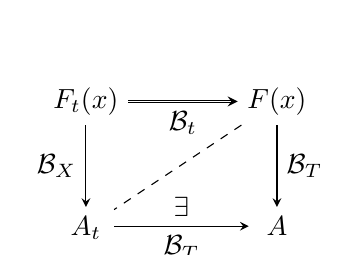
\begin{tikzpicture}
  \matrix (m) [matrix of math nodes,row sep=3em,column sep=4em,minimum width=2em]
  {
     F_t(x) & F(x) \\
     A_t & A \\};
  \path[-stealth]
    (m-1-1) edge node [left] {$\mathcal{B}_X$} (m-2-1)
            edge [double] node [below] {$\mathcal{B}_t$} (m-1-2)
    (m-2-1.east|-m-2-2) edge node [below] {$\mathcal{B}_T$}
            node [above] {$\exists$} (m-2-2)
    (m-1-2) edge node [right] {$\mathcal{B}_T$} (m-2-2)
            edge [dashed,-] (m-2-1);
\end{tikzpicture}
\end{center}

\todo{Bundle maps, when reduced structure group, Berger's list}


\subsection{Compactification on Calabi-Yau}
Having reviewed the notion of reduced structure group and special holonomy a Calabi-Yau n-fold $CY_{n}$ can be defined as a $2n$-dimensional compact Riemannian manifolds with holonomy contained in $SU(N)$\cite{Blumenhagen2013}. We are particularly interested in $CY_3$ such that starting in $D=10$ supergravity, or string theory, the external spacetime is 4-dimensional. As such we know that for a $CY_3$ there exists some invariant p-forms which can be found by looking at the decomposition of 1-,2- and 3-forms of $SO(6)\cong SU(4)$ under $\mathcal{H}=SU(3)$
\begin{align*}
    \mathbf{6}\to \mathbf{3}+\mathbb{\overbar{3}},\\
    \mathbf{15}\to \mathbf{8}+\mathbb{3}+\overbar{\mathbf{3}}+\mathbf{1},\\
    \mathbf{20}\to \mathbf{6}+\overbar{\mathbf{6}}+\mathbf{3}+\overbar{\mathbf{3}}+2\cdot\mathbf{1}.
\end{align*}
There thus exists a real 2-form $\omega$ and a complex 3-form $\Omega$ that are singlets under $\mathcal{H}$, such pair of nowhere vanishing tensors defines a \emph{structure}. Note that we already know that such a structure is equally well defined by a nowhere globally defined spinor $\mathbb{4}$ of $SU(4)\cong SO(6)$ that decomposes under $\mathcal{H}$ as 
\begin{equation}
    \mathbf{4}\to \mathbf{3}+\mathbf{1}.
\end{equation}
What follows will mostly consider structures defined by some bosonic forms such as ($\omega,\Omega$) but from the observation above we know that this corresponds to a Killing spinor which in turn depends on preserving some amount of supersymmetry. Moreover, we see that starting with $\mathcal{N}$ supersymmetries in the full theory compactification on a $CY_3$ yields a theory which again has $\mathcal{N}$ supersymmetries.

\section{Flux compactifications and generalised geometry}
In the case of vanishing flux we have seen that the Killing spinor equation led to special holonomy, which in put restrictions on the connection of the internal manifold. In the presence of fluxes the Killing spinor is no longer covariantly constant, however, the existence of globally defined nowhere vanishing spinor still implies a reduced structure group. This is summarized by 

\begin{align*}
    \text{vanishing flux}&\Longleftrightarrow \text{special holonomy},\\
    \text{non-zero flux}&\Longleftrightarrow \text{reduced structure group}.\\
\end{align*}
In the presence of fluxes the Killing spinor equations of type II supergravity are given by \cite{Blumenhagen2013}
\begin{equation}
    \delta_\epsilon \psi_M = \left(\nabla_M+\frac{1}{8}\Gamma^{NP}H_{MNP}\mathscr{P}+\frac{1}{16}\ee^\Phi\sum_{n}\slashed{F}_n\Gamma_M\mathscr{P}_n\right)\epsilon,
\end{equation}
\begin{equation}
    \delta_\epsilon \lambda = \left(\slashed{\pd}\Phi+\frac{1}{12}\Gamma^{MNP}H_{MNP}\mathscr{P}+\frac{1}{8}\ee^\Phi\sum_{n}(-1)^n(5-n)\slashed{F}_n\mathscr{P}_n\right)\epsilon,
\end{equation}
where $\mathscr{P}$ and $\mathscr{P_n}$ are $2\times 2$-matrices, $\slashed{F}_n=\frac{1}{n!}\Gamma^{M_1M_2\ldots M_n}F_{M_1M_2\ldots M_n}$ and $n\in\{0,1,\ldots,10\}$ is even(odd) for type IIA(B). In the case of vanishing flux and a constant dilation this is seen to reduce to a covariantly constant spinor $\epsilon$ as discussed above. 

The obstruction to the Killing spinor being covariantly constant is typically discussed in terms of intrinsic torsion. However, there is always possible to construct a connection $\nabla$ with torsion such that the Killing spinor is covariantly constant w.r.t. to that connection. Thus consider a connection $\nabla=\nabla'-\kappa$ such that $\nabla_n V_m=\pd_nV_m-\tensor{\Gamma}{^'_{nm}^p}V_p-\tensor{\kappa}{_{nm}^p}V_p$, where $\nabla'$ is the Levi-Civita connection and $\kappa$ is the so-called contorsion tensor. Generically the connection coefficents $\tensor{\Gamma}{_{mn}^p}$ take values in $\Lambda^1\otimes\mathfrak{g}$, where $\lambda^1$ is the one-form representation of $G=GL(d)$ and $\mathfrak{g}=\mathfrak{gl}(d)$ is the corresponding Lie algebra. Assuming metric compatibility fixes the ``symmetric'' part of the pair $_m^p$ which is contained in the Levi-connection. Note that the Levi-Civita connection have extra terms such that the torsion $\tensor{\Gamma}{_{[mn]^p}}$ vanishes. This implies that the contorsion take values in 
\begin{equation}
    \tensor{\kappa}{_{mn}^p}\in \Lambda_1\otimes \mathfrak{h},
\end{equation}
where $\mathfrak{h}=so(d)$ is the maximal compact subalgebra of $\mathfrak{gl}(d)$ (since this is the ``anti-symmetric'' part). Assuming a reduced structure group $G'\subseteq SO(d)$ implies that we can separate the contorsion into two parts 
\begin{equation}
    \kappa = \kappa_0+\kappa_{\text{int}}\quad \text{where} \quad \kappa_{\text{int}}\in \Lambda_1\otimes \mathfrak{g}'\quad \text{and}\quad \kappa_{0}\in \Lambda_1\otimes \tensor{\mathfrak{g}}{^'^{\perp}}.
\end{equation}
The point now being that since the Killing spinor is a singlet under $G'$ the failure of the of Killing spinor being covariantly constant \emph{with respect to the Levi-Civita connection} is given by $\kappa_0$. The part $\kappa_0$ can further be decomposed into irreducible representations of $\mathfrak{g}'$ called torsion classes. As an example take $G=GL(6)$ and $G'=SU(3)$. Under $G'$ we have the following decompositions $\Lambda_1\to \mathbf{3}\oplus\overbar{\mathbf{3}}$, $\mathfrak{g}'=\mathbf{8}$ and $\tensor{\mathfrak{g}}{^'^{\perp}}=\mathbf{1}\oplus\mathbf{3}\oplus\overbar{\mathbf{3}}$ and 
\begin{equation}
    \kappa_0 \in \bigoplus_{i=1}^5 \mathscr{W}_i,
\end{equation}
where $\mathscr{W}_i$ are the five torsion classes given by 
\begin{align*}
    \mathscr{W}_1 = \mathbf{1}\oplus\mathbf{1},\\
    \mathscr{W}_2 = \mathbf{8}\oplus\mathbf{8},\\
    \mathscr{W}_3 = \mathbf{6}\oplus\overbar{\mathbf{6}},\\
    \mathscr{W}_4 = \mathbf{3}\oplus\overbar{\mathbf{3}}.\\
\end{align*}








\chapter{Summary}


% REFERENCES / BIBLIOGRAPHY
\cleardoublepage
\addcontentsline{toc}{chapter}{Bibliography}
\printbibliography

% APPENDICES
\cleardoublepage
\appendix
\setcounter{page}{1}
\pagenumbering{Roman}			% Capitalized roman numbering starting from I (one)

\chapter{Closure of generalised diffeomorphisms}
%Lorem ipsum dolor sit amet, consectetur adipisicing elit, sed do eiusmod tempor incididunt ut labore et dolore magna aliqua. Ut enim ad minim veniam, quis nostrud exercitation ullamco laboris nisi ut aliquip ex ea commodo consequat. Duis aute irure dolor in reprehenderit in voluptate velit esse cillum dolore eu fugiat nulla pariatur. Excepteur sint occaecat cupidatat non proident, sunt in culpa qui officia deserunt mollit anim id est laborum.

%\section{Momentum maps and conserved quantities}
https://arxiv.org/pdf/physics/9801019.pdf
\todo{examples such as the bosonic string, Noether's theorem}
\section{Closure of generalised diffeomorphisms\label{app:GenDiffComm}}
In this appendix we provide the explicit calculation of closure of generalised diffeomorphisms. We want to look at $[\mathscr{L}_\xi,\mathscr{L}_\eta] V^M$ and start with one term 
\begin{equation}
    \begin{aligned}
        \mathscr{L}_{\xi}(\mathscr{L}_\eta V^M) &= \mathscr{L}_\xi(\eta^P\pd_PV^M-\pd_P\eta^MV^P+\tensor{Y}{^{MR}_{ST}}\pd_R\eta^S V^T)\\
        &= (\mathscr{L}_\xi \eta^P)\pd_PV^M+\eta^P\mathscr{L}_\xi(\pd_PV^M)-(\mathscr{L}_\xi\pd_P\eta^M)V^P-\pd_P\eta^M\mathscr{L}_\xi V^P\\
        &+\tensor{Y}{^{MR}_{ST}}(\mathscr{L}_\xi\pd_R\eta^S)V^T+\tensor{Y}{^{MR}_{ST}}\pd_R\eta^S\mathscr{L}_\xi V^T.
    \end{aligned}
\end{equation}
The first term gives 
\begin{equation}
    \begin{aligned}
        (\mathscr{L}_\xi\eta^P)\pd_PV^M &= \xi^K\pd_K\eta^P\pd_PV^M-\pd_K\xi^M\pd_PV^K+\pd_K\xi^K\pd_KV^M\\
        &+\tensor{Y}{^{MR}_{ST}}(\pd_R\xi^S)\pd_PV^T-\underbrace{\tensor{Y}{^{TR}_{SP}}(\pd_R\xi^S)\pd_TV^M}_{=0\,\text{section condition}}.
    \end{aligned}
\end{equation}
The second term gives 
\begin{equation}
    \begin{aligned}
        \eta^P(\mathscr{L}_\xi\pd_PV^M) &= \eta^P\xi^K\pd_K\pd_PV^M-\eta^P\pd_K\xi^M\pd_PV^K+\eta^P\pd_P\xi^K\pd_KV^M\\
        &+ \tensor{Y}{^{MR}_{ST}}(\pd_R\xi^S)\pd_PV^T-\underbrace{\tensor{Y}{^{TR}_{SP}}(\pd_R\xi^S)\pd_TV^M}_{=0\, \text{section condition}},
    \end{aligned}
\end{equation}
where we note that the first terms is symmetric in $\xi\leftrightarrow\eta$ and will vanish in the commutator. The third term gives 
\begin{equation}
    \begin{aligned}
        -(\mathscr{L}_\xi\pd_PV^M)V^P&=-\xi^K\pd_K\pd_P\eta^MV^P+\pd_K\xi^M\pd_P\eta^KV^P-\pd_P\xi^K\pd_K\eta^MV^P\\
        &-\tensor{Y}{^{MR}_{ST}}(\pd_R\xi^S)\pd_\eta^TV^P+\underbrace{\tensor{Y}{^{TR}_{SP}}(\pd_R\xi^S)\pd_TV^P}_{=0\, \text{section condition}}.
    \end{aligned}
\end{equation}
The fourth term is given by 
\begin{equation}
    -\pd_P\eta^M\mathscr{L}_\xi V^P = -\pd_\eta^M\xi^K\pd_KV^P+\pd_P\eta^M\pd_K\xi^PV^K-\underbrace{\pd_P\eta^M\tensor{Y}{^{PR}_{ST}}(\pd_R\xi^S)\pd_P\eta^M}_{=0\, \text{section condition}}.
\end{equation}
The fifth term is given by 
\begin{equation}
    \begin{aligned}
        \tensor{Y}{^{MR}_{ST}}(\mathscr{L}_\xi \pd_R\eta^S)V^T &= \tensor{Y}{^{MR}_{ST}}V^T\left(\xi^K\pd_K\pd_R\eta^S-\pd_K\xi^S\pd_R\eta^K+\pd_R\xi^K\pd_K\eta^S\right)\\
        &+\tensor{Y}{^{MR}_{ST}}V^T\big(\tensor{Y}{^{SK}_{LQ}}(\pd_K\xi^L)\pd_R\eta^Q-\underbrace{\tensor{Y}{^{QK}_{LR}}(\pd_K\xi^L)\pd_Q\eta^S}_{=0\, \text{section condition}}\big).
    \end{aligned}
\end{equation}
And finally the last term is given by 
\begin{equation}
    \begin{aligned}
        \tensor{Y}{^{MR}_{ST}}(\pd_R\eta^S)\mathscr{L}_\xi V^T = \tensor{Y}{^{MR}_{ST}}\left(\pd_R\eta^S\xi^K\pd_KV^T-\pd_K\xi^TV^K+\tensor{Y}{^{TK}_{QP}}(\pd_K\xi^Q)V^P\right).
    \end{aligned}
\end{equation}
We also want to calculate $\frac{1}{2}(\mathscr{L}_{\mathscr{L}_\xi\eta}-\mathscr{L}_{\mathscr{L}_\eta\xi})V^M$ to this end calculate
\begin{equation}
    \mathscr{L}_{\mathscr{L}_\xi \eta}V^M = \mathscr{L}_{\xi^K\pd_K\eta}V^M-\mathscr{L}_{\pd_K\xi\eta^K}V^M+\mathscr{L}_{\tensor{Y}{^{\circ R}_{ST}}\pd_R\xi^S\eta^T}V^M.
\end{equation}
The first term gives 
\begin{equation}
    \begin{aligned}
        \mathscr{L}_{\xi^K\pd_K\eta}V^M &= \xi^K\pd_K\eta^P\pd_PV^M-\left(\pd_P\xi^K\pd_K\eta^M+\xi^K\pd_K\pd_P\eta^M\right)V^P\\
        &+\tensor{Y}{^{MR}_{ST}}\left(\pd_\xi^K\pd_K\eta^S+\xi^K\pd_K\pd_R\eta^S\right)V^T.
    \end{aligned}
\end{equation}
The second term gives 
\begin{equation}
    \begin{aligned}
        -\mathscr{L}_{\pd_K\xi\eta^K}V^M &= -\pd_K\xi^P\eta^K\pd_PV^M+\left(\eta^K\pd_K\pd_P\xi^M+\pd_K\xi^M\pd_P\eta^K\right)V^P\\
        &-\tensor{Y}{^{MR}_{ST}}\left(\pd_R\pd_K\xi^S\eta^K+\pd_K\xi^S\pd_R\eta^K\right)V^T.
    \end{aligned}
\end{equation}
And the last term gives 
\begin{equation}
    \begin{aligned}
        \mathscr{L}_{\tensor{Y}{^{\circ R}_{ST}}\pd_R\xi^S\eta^T}V^M &= \underbrace{\tensor{Y}{^{KR}_{ST}}(\pd_R\xi^S)\eta^T\pd_KV^M}_{=0\, \text{section condition}}-\tensor{Y}{^{MR}_{ST}}V^K\left(\pd_K\pd_R\xi^S\eta^T+\pd_R\xi^S\pd_K\eta^T\right)\\
        &+\tensor{Y}{^{MQ}_{LK}}\tensor{Y}{^{LR}_{ST}}V^K\left(\pd_Q\pd_R\xi^S\eta^T+\pd_R\xi^S\pd_Q\eta^T\right).
    \end{aligned}
\end{equation}
It is then straightforward but tedious to calculate $[\mathscr{L}_\xi,\mathscr{L}_\eta] V^M-\frac{1}{2}(\mathscr{L}_{\mathscr{L}_\xi\eta}-\mathscr{L}_{\mathscr{L}_\eta\xi})V^M$ and one finds that the contribution from the terms proportional to $\pd^2\xi$ is given by
\begin{equation}
    \frac{1}{2}\left(\tensor{Y}{^{MR}_{ST}}\pd_K\pd_R\xi^S-\tensor{Y}{^{MQ}_{LK}}\tensor{Y}{^{LR}_{ST}}\pd_Q\pd_R\xi^S\right)V^K\eta^T = -\frac{1}{2}\tensor{Z}{^{MQ}_{LK}}\tensor{Y}{^{LR}_{ST}}\pd_Q\pd_R\xi^SV^T\eta^K,
\end{equation}
which is not but an anciallary transformation. The remaining terms are proportional to $(\pd\xi\pd\eta)$ and given by 
\begin{equation}
    \begin{aligned}
        \frac{1}{2}\tensor{Y}{^{MR}_{ST}}\tensor{Y}{^{SK}_{LQ}}\pd_K\xi^L\pd_R\eta^QV^T+\tensor{Y}{^{MR}_{ST}}\tensor{Y}{^{TK}_{QP}}\pd_R\eta^S\pd_K\xi^QV^P\\
        -\frac{1}{2}\tensor{Y}{^{MR}_{ST}}\pd_K\xi^T\pd_R\eta^SV^K-\tensor{Y}{^{MR}_{ST}}\pd_K\xi^S\pd_R\eta^KV^T-(\xi\leftrightarrow\eta) \overset{!}{=}0.
    \end{aligned}
\end{equation}
The identities that the $Y$ tensor need to satisfy given in \eqref{eq:closure1}-\eqref{eq:closure2} are then easily derived from this expression. 



\end{document} 
